\subsubsection{Logistic map (LOG)} \label{subsubsec:log}

Logistic map is representative of the very large family of quadratic maps. 
\begin{equation}\label{eq:logimap}
 x_{[n+1]}=4x_{[n]}(1-x_{[n]}) \,
\end{equation}
with $x_n\in\mathcal{R}$.

Note that to effectively work in a given representation it is necessary to change the expression of the map in order to make all the operations in the chosen representation numbers. For example, in the case of LOG the expression in binary fixed point numbers is:
\begin{equation}\label{eq:logimapB2}
x_{n+1}=4 \epsilon floor\{\frac{x_n(1-x_n)}{\epsilon}\} \,
\end{equation}
with $\epsilon = 2^B$ where $B$ is the length of fractional part.

Figs. \ref{fig:LOG_QuantiB} (a) to (f) show the statistical properties of LOG map in floating point and fixed point representation.
All these figures shows: in red dots the results of each run (100 point for each presicion), in black dots the mean of these 100 points (dashed black line connects black dots), in dashed blue lines the results of each run in floating point and (100 horizontal blue dashed lines) and in black the mean for floating point.

For $B\geq 30$ the value of $H_{val}$ remains almost identical to the values for the floating point representation whereas $H_{BP}$ and $C_{BP}$ stabilizes at $B>21$.
Their values are: $<H_{val}>=0.9669$; $<H_{BP}>=0.6269$; $<C_{BP}>=0.4843$.
Note that the stable value of missing patterns $645$ makes the optimum $H_{BP} \leq ln(75)/ln(720) \simeq 0.65$, this value of $MP$ is reached for $B>21$, the same of $<H_{BP}>=0.6269$ and $<C_{BP}>=0.4843$.
Then $B=30$ is the most convenient choice because an increase in the number of fractional figures does not improve the statistical properties.

We can extract some conclussions when compare \textit{BP} with \textit{BPW} quantifiers.
We can see that for $B=1, 2, 3 and 4$, $BP$ quantifiers is almost $0$ and $BPW$ quantifiers not exists in the mean, the initial condition of some atractors was rounded to $0$ and $BPW$ histogram not exist.
For $B=7, 9 and 12$, an high dispersion in $BPW$ are showed, but not in $BP$ graphs, atractor falls to a fixed point with an short transitory in these cases.
Finally, for $B = 45, 49, 51 and 52$ some $BP$ quantifiers has a low value, but $BPW$ quantifiers has a more predictible behavior, we can see that these atractors falls to a fixed point with a long trnsitory.
In this case the problem has to do with the plataform that we use, the miltiplication needs the double of bits to be represented but the machine has only $64$.

\begin{figure}
	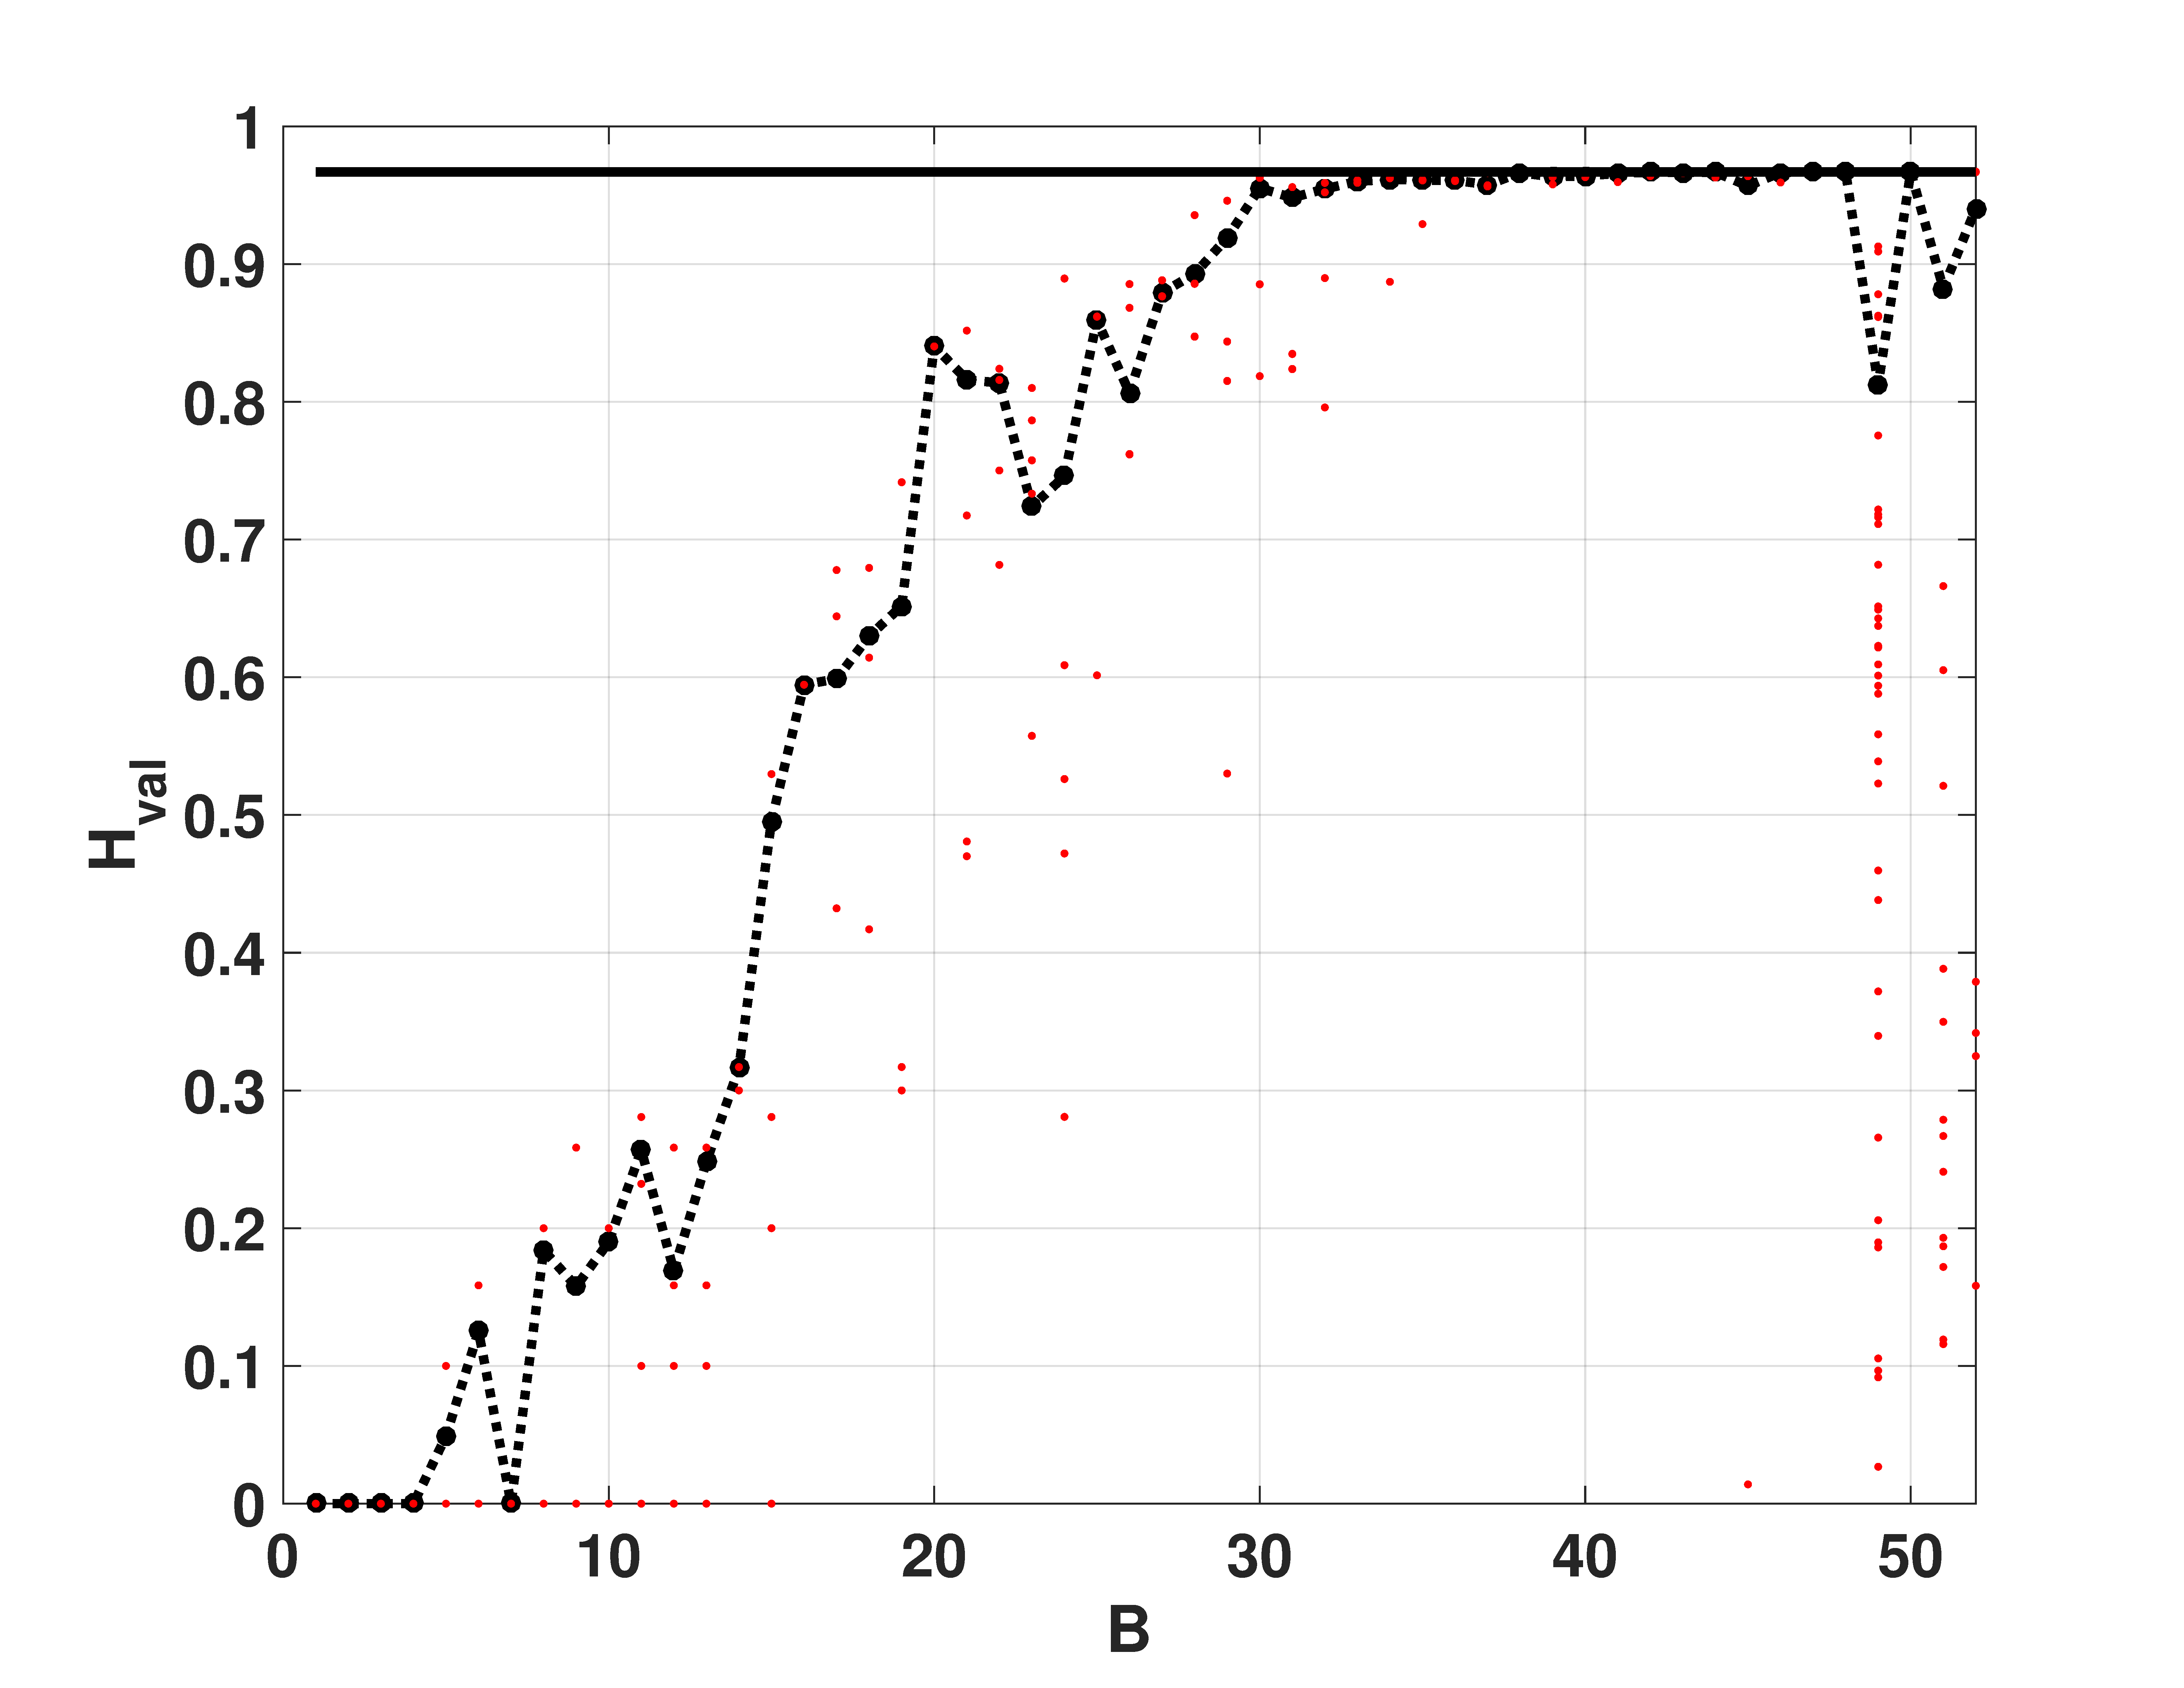
\includegraphics[width= .49\textwidth]{Hval_Logistico}
	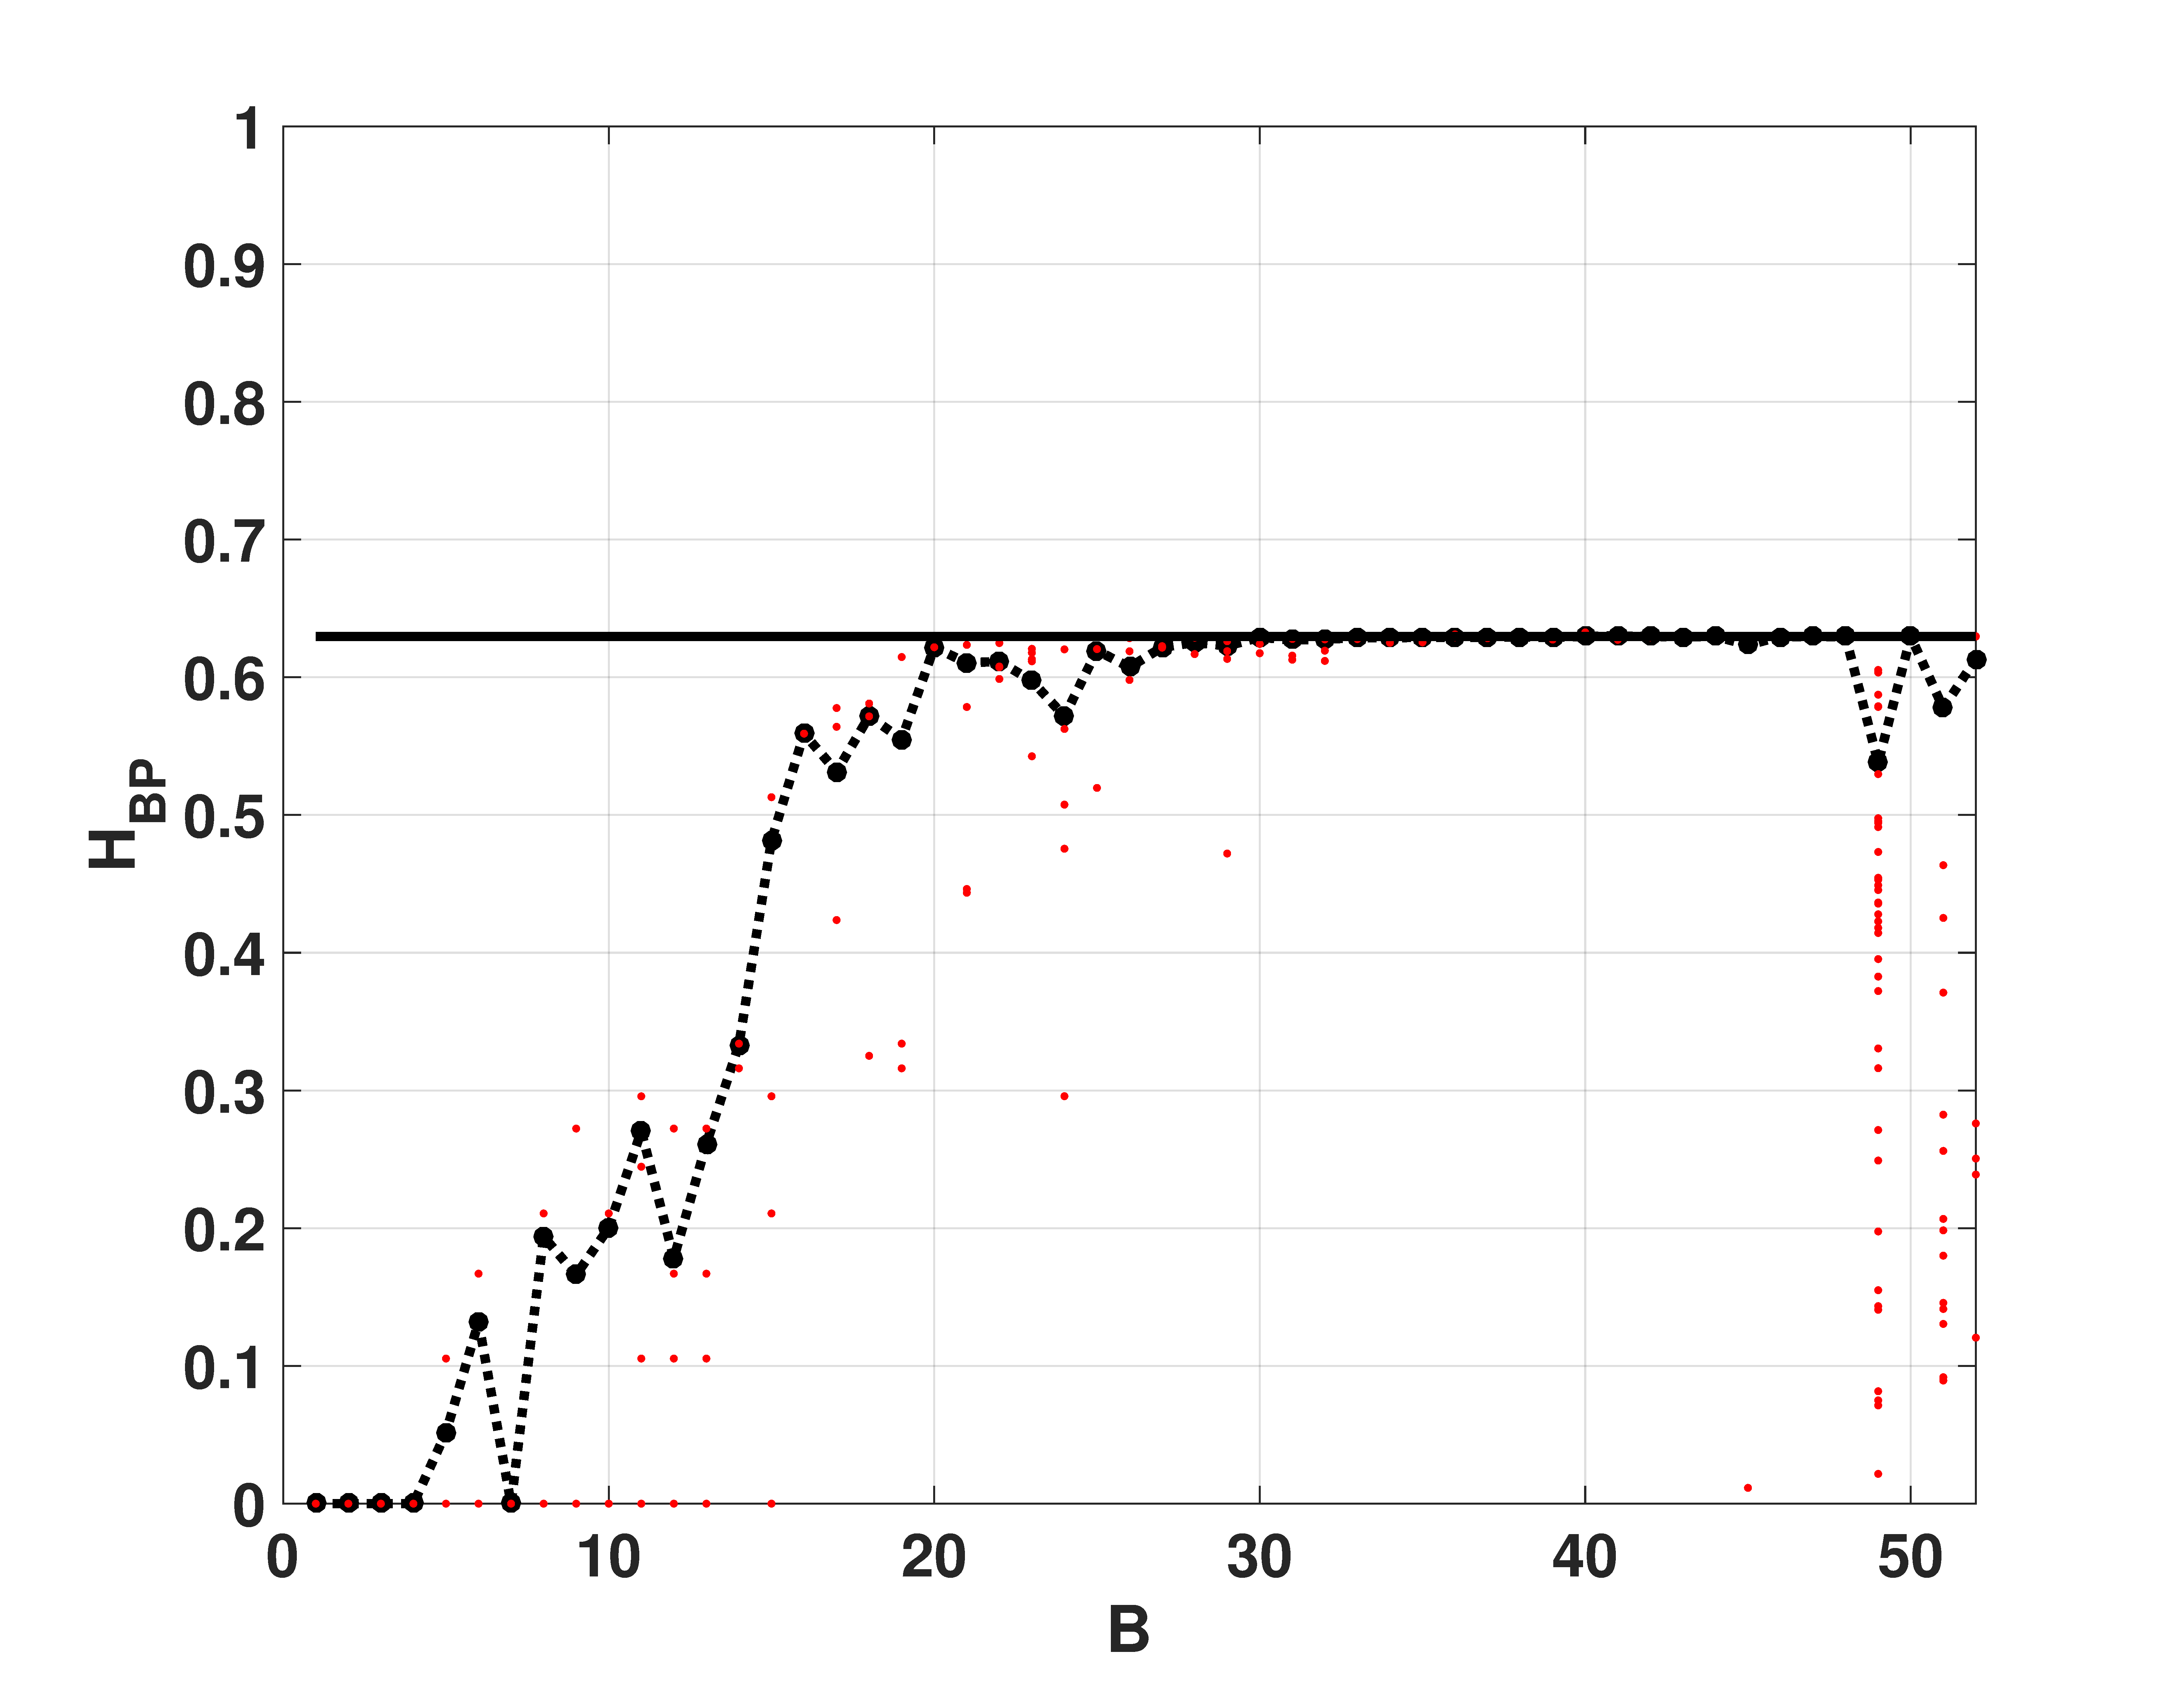
\includegraphics[width= .49\textwidth]{Hbp_Logistico}
	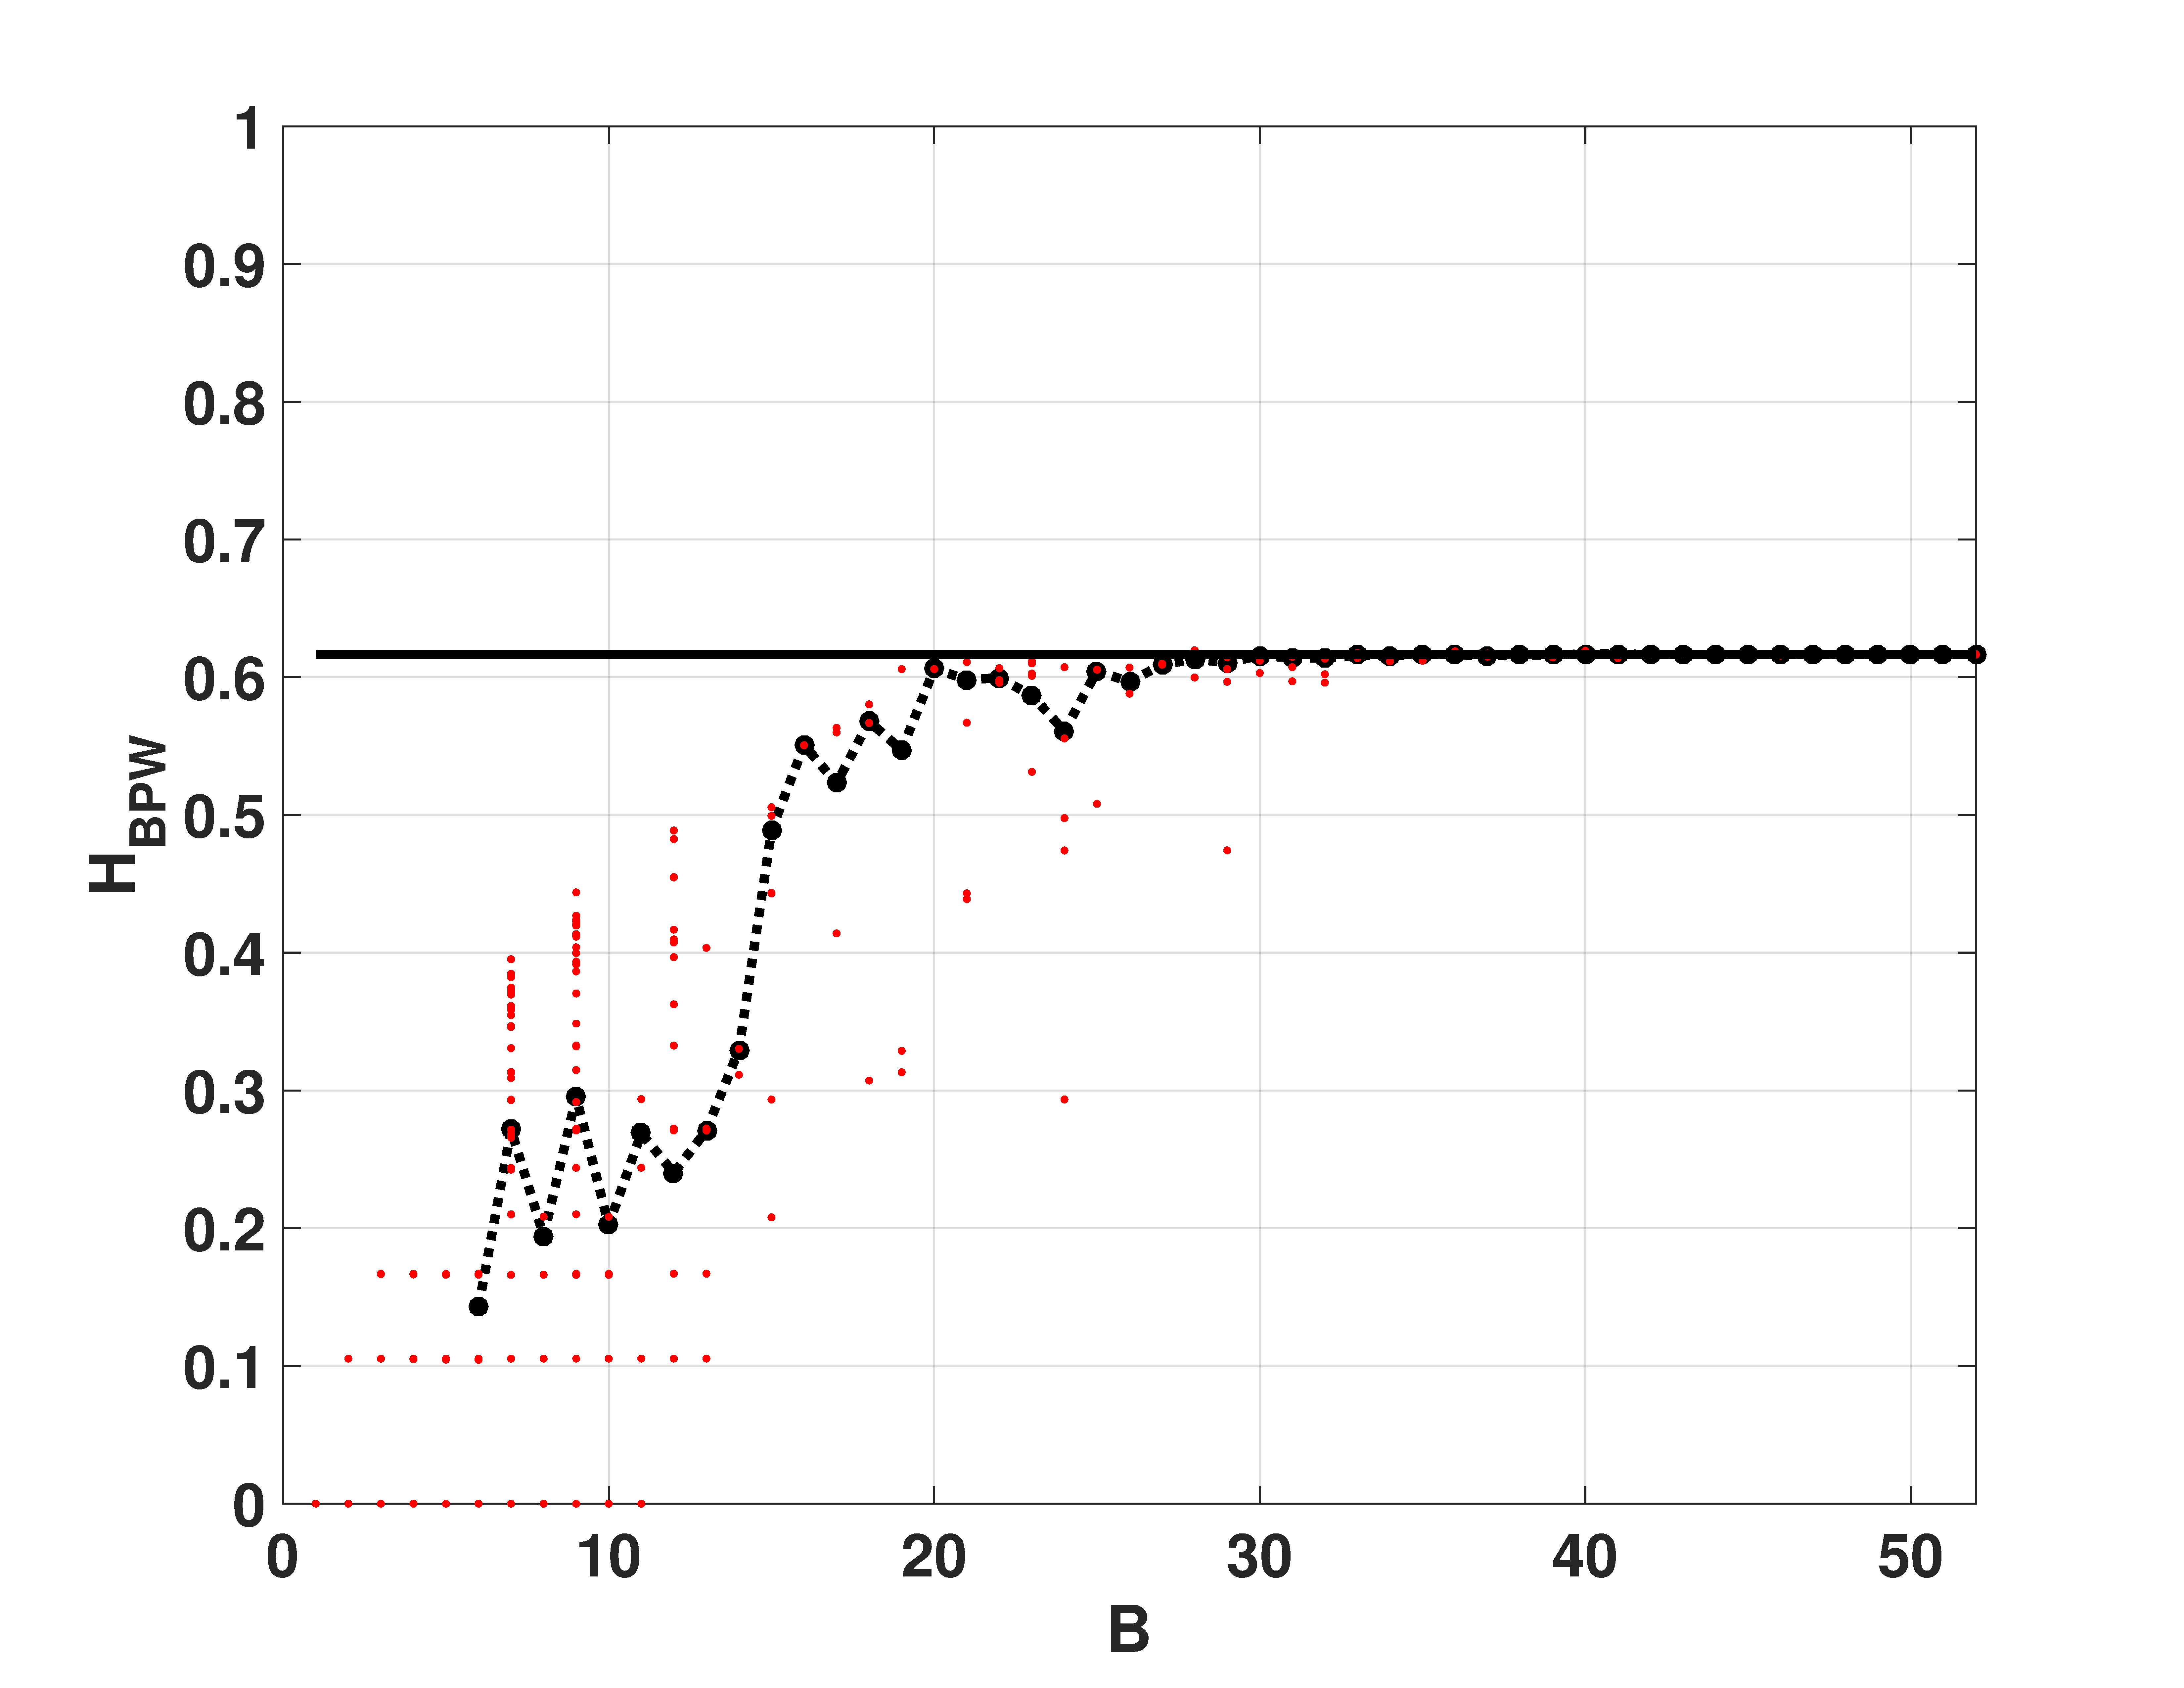
\includegraphics[width= .49\textwidth]{Hbpw_Logistico}
	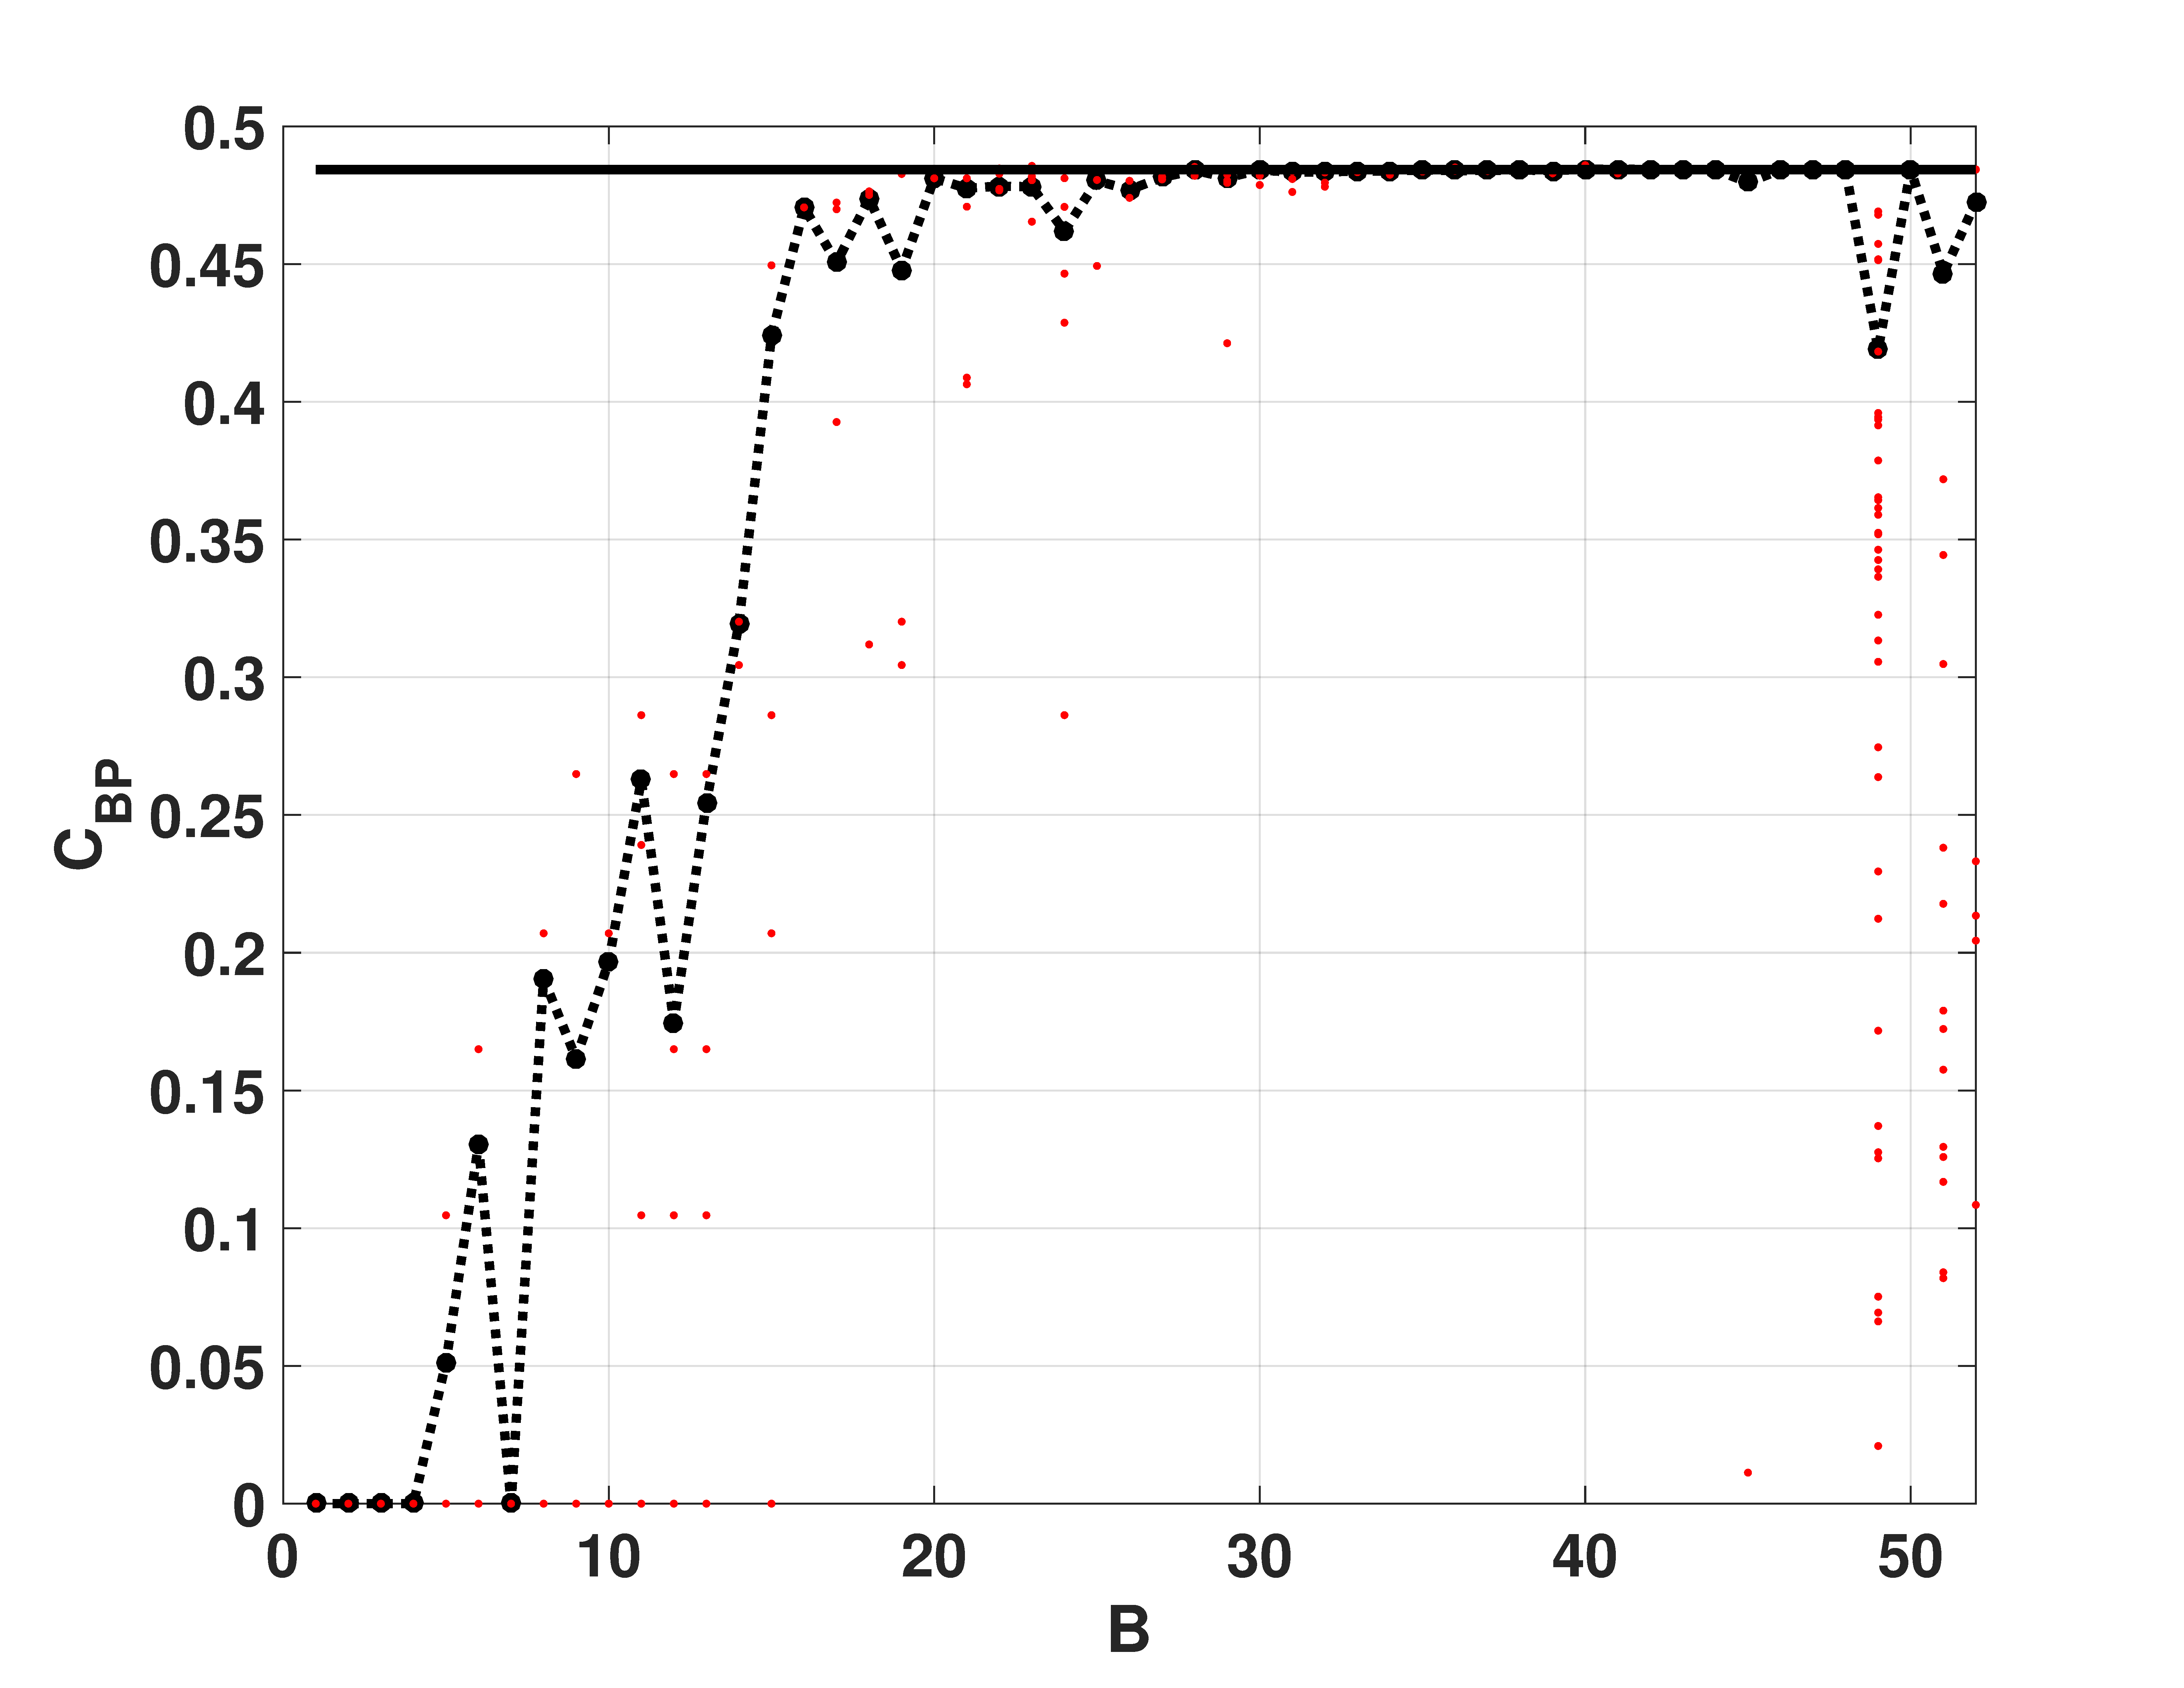
\includegraphics[width= .49\textwidth]{Cbp_Logistico}
	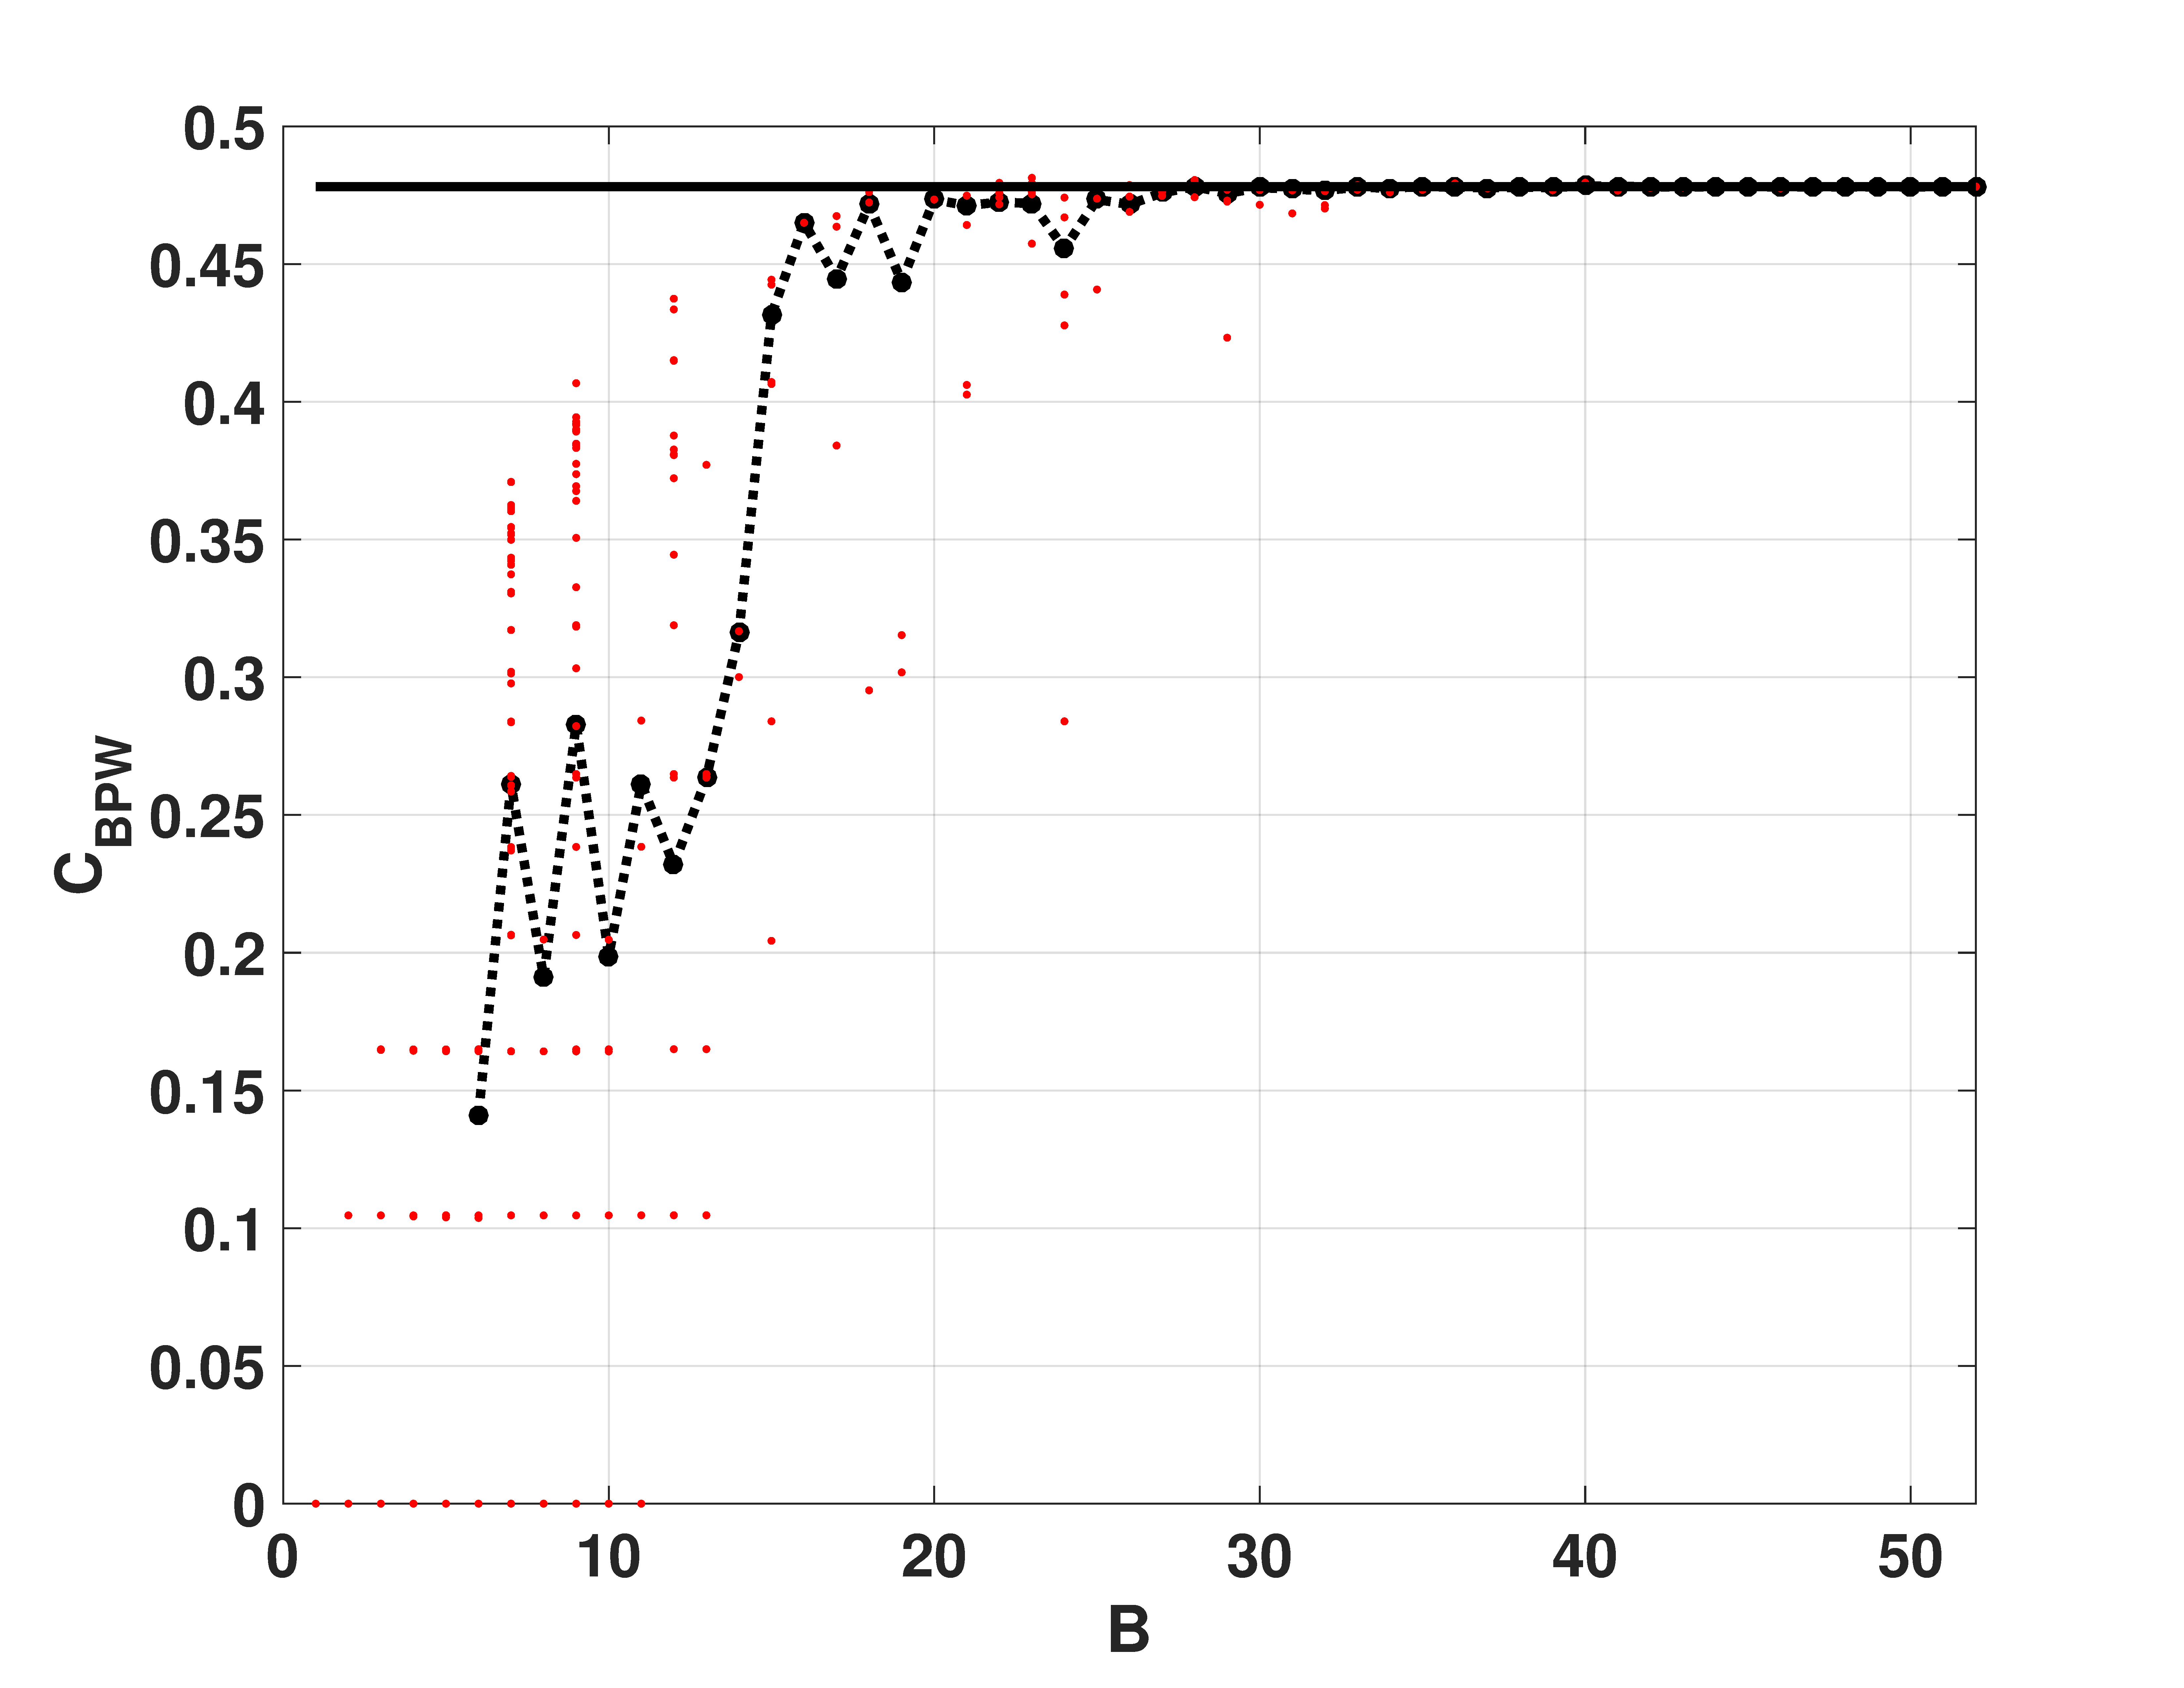
\includegraphics[width= .49\textwidth]{Cbpw_Logistico}
	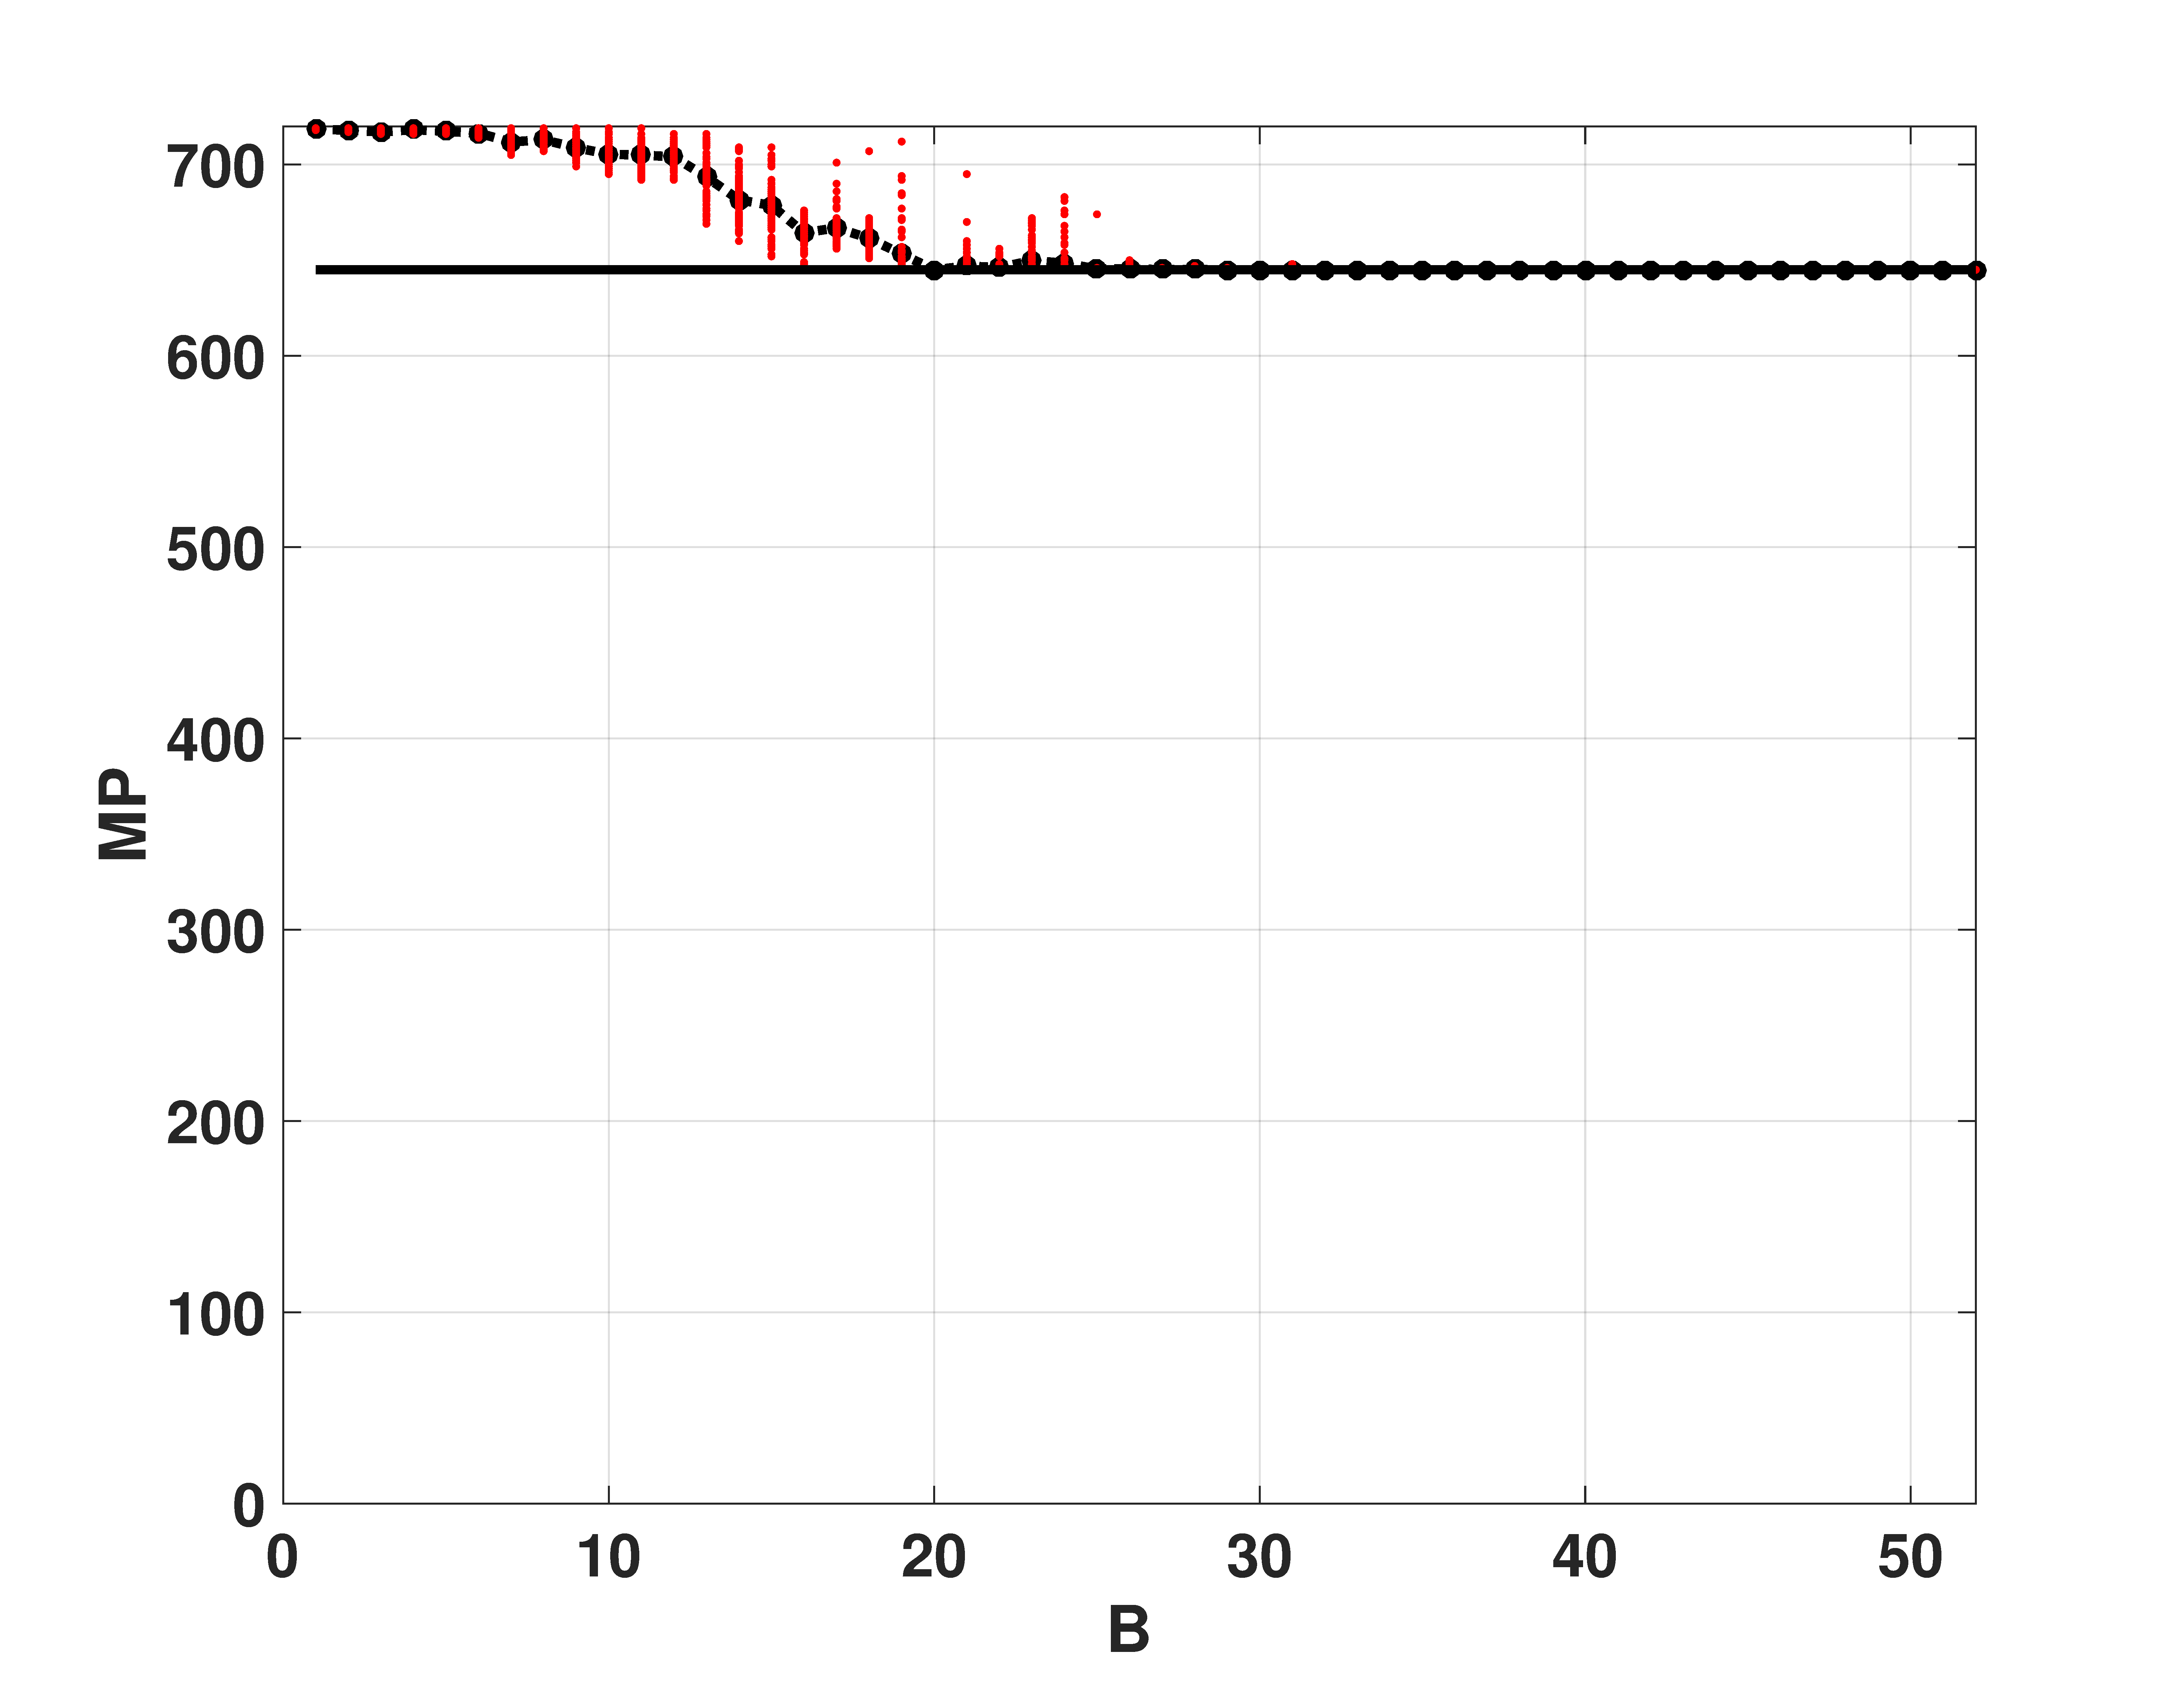
\includegraphics[width= .49\textwidth]{MP_Logistico}
	\caption{Statistical properties of the LOG map using binary representation: (a) $H_{hist}$ vs $P$ (b) $H_{BP}$ vs $P$ (c) $C_{BP}$ vs $P$ (d) Number of missing ordering patterns $MP$ vs $P$. In Figures (a) to (d) dashed line correspond to floating point numbers. (d) representation in the $H_{hist},H_{BP}$ plane in the the decimal numerical system.  The star represents the state for floating points numbers. (e) representation in the $H_{hist},H_{BP}$ plane. The star represents the state for floating point numbers; (f) representation in the $H_{BP},C_{BP}$ plane.  The star represents the state for floating points numbers. (f) representation in the $H_{BP},C_{BP}$ plane for binary numerical system.  The star represents the state for floating points numbers. } \label{fig:LOG_QuantiB}
\end{figure}

In Fig. \ref{fig:LOG_HH} double entropy planes are showed.
Red points are each individual measurement and black points their mean.
Black dashed line shows the evolution of the mean in this plane when $B$ growths.
Blue points shows each individual measurement in floating point and their mean with an star.

Although the distribution of values reaches high values, their mixing is poor.
It can be seen in the evolution of the mean values according $B$ growths.
Accross $B=20$, $H_{val}$ improves but $H_{BP}$ stay around its maximum.

\begin{figure}
	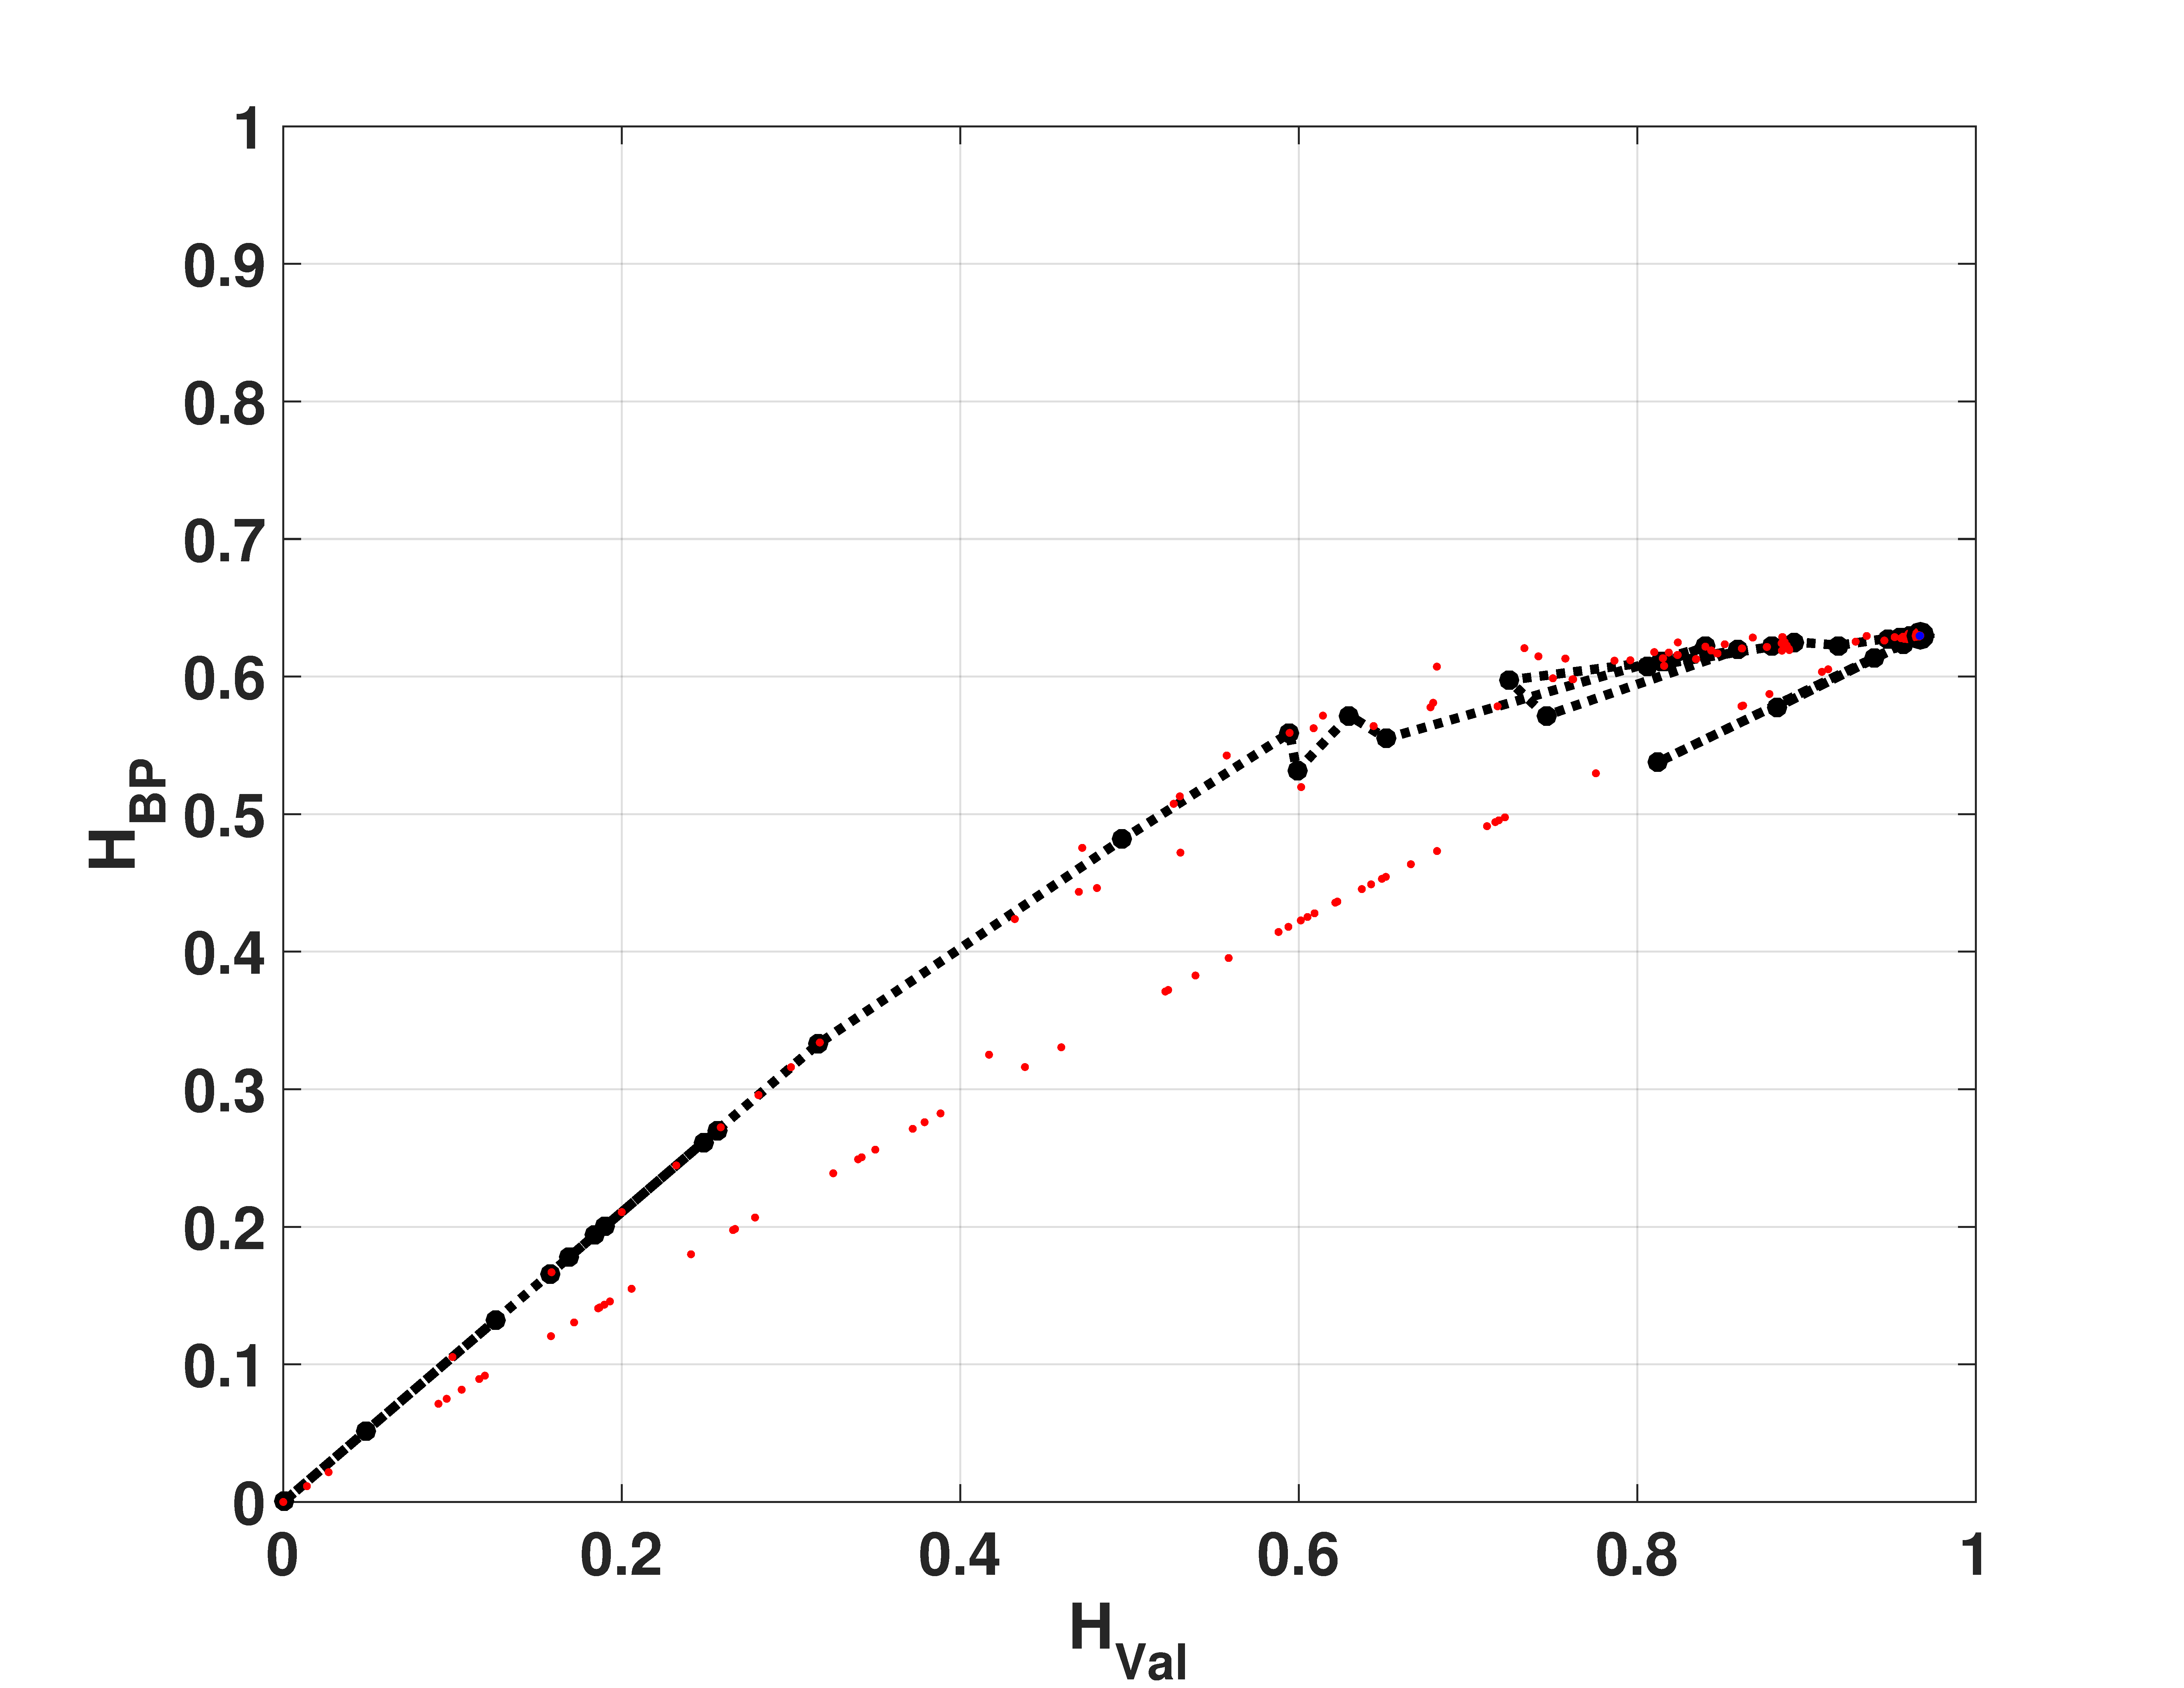
\includegraphics[width= .49\textwidth]{HbpHval_Logistico}
	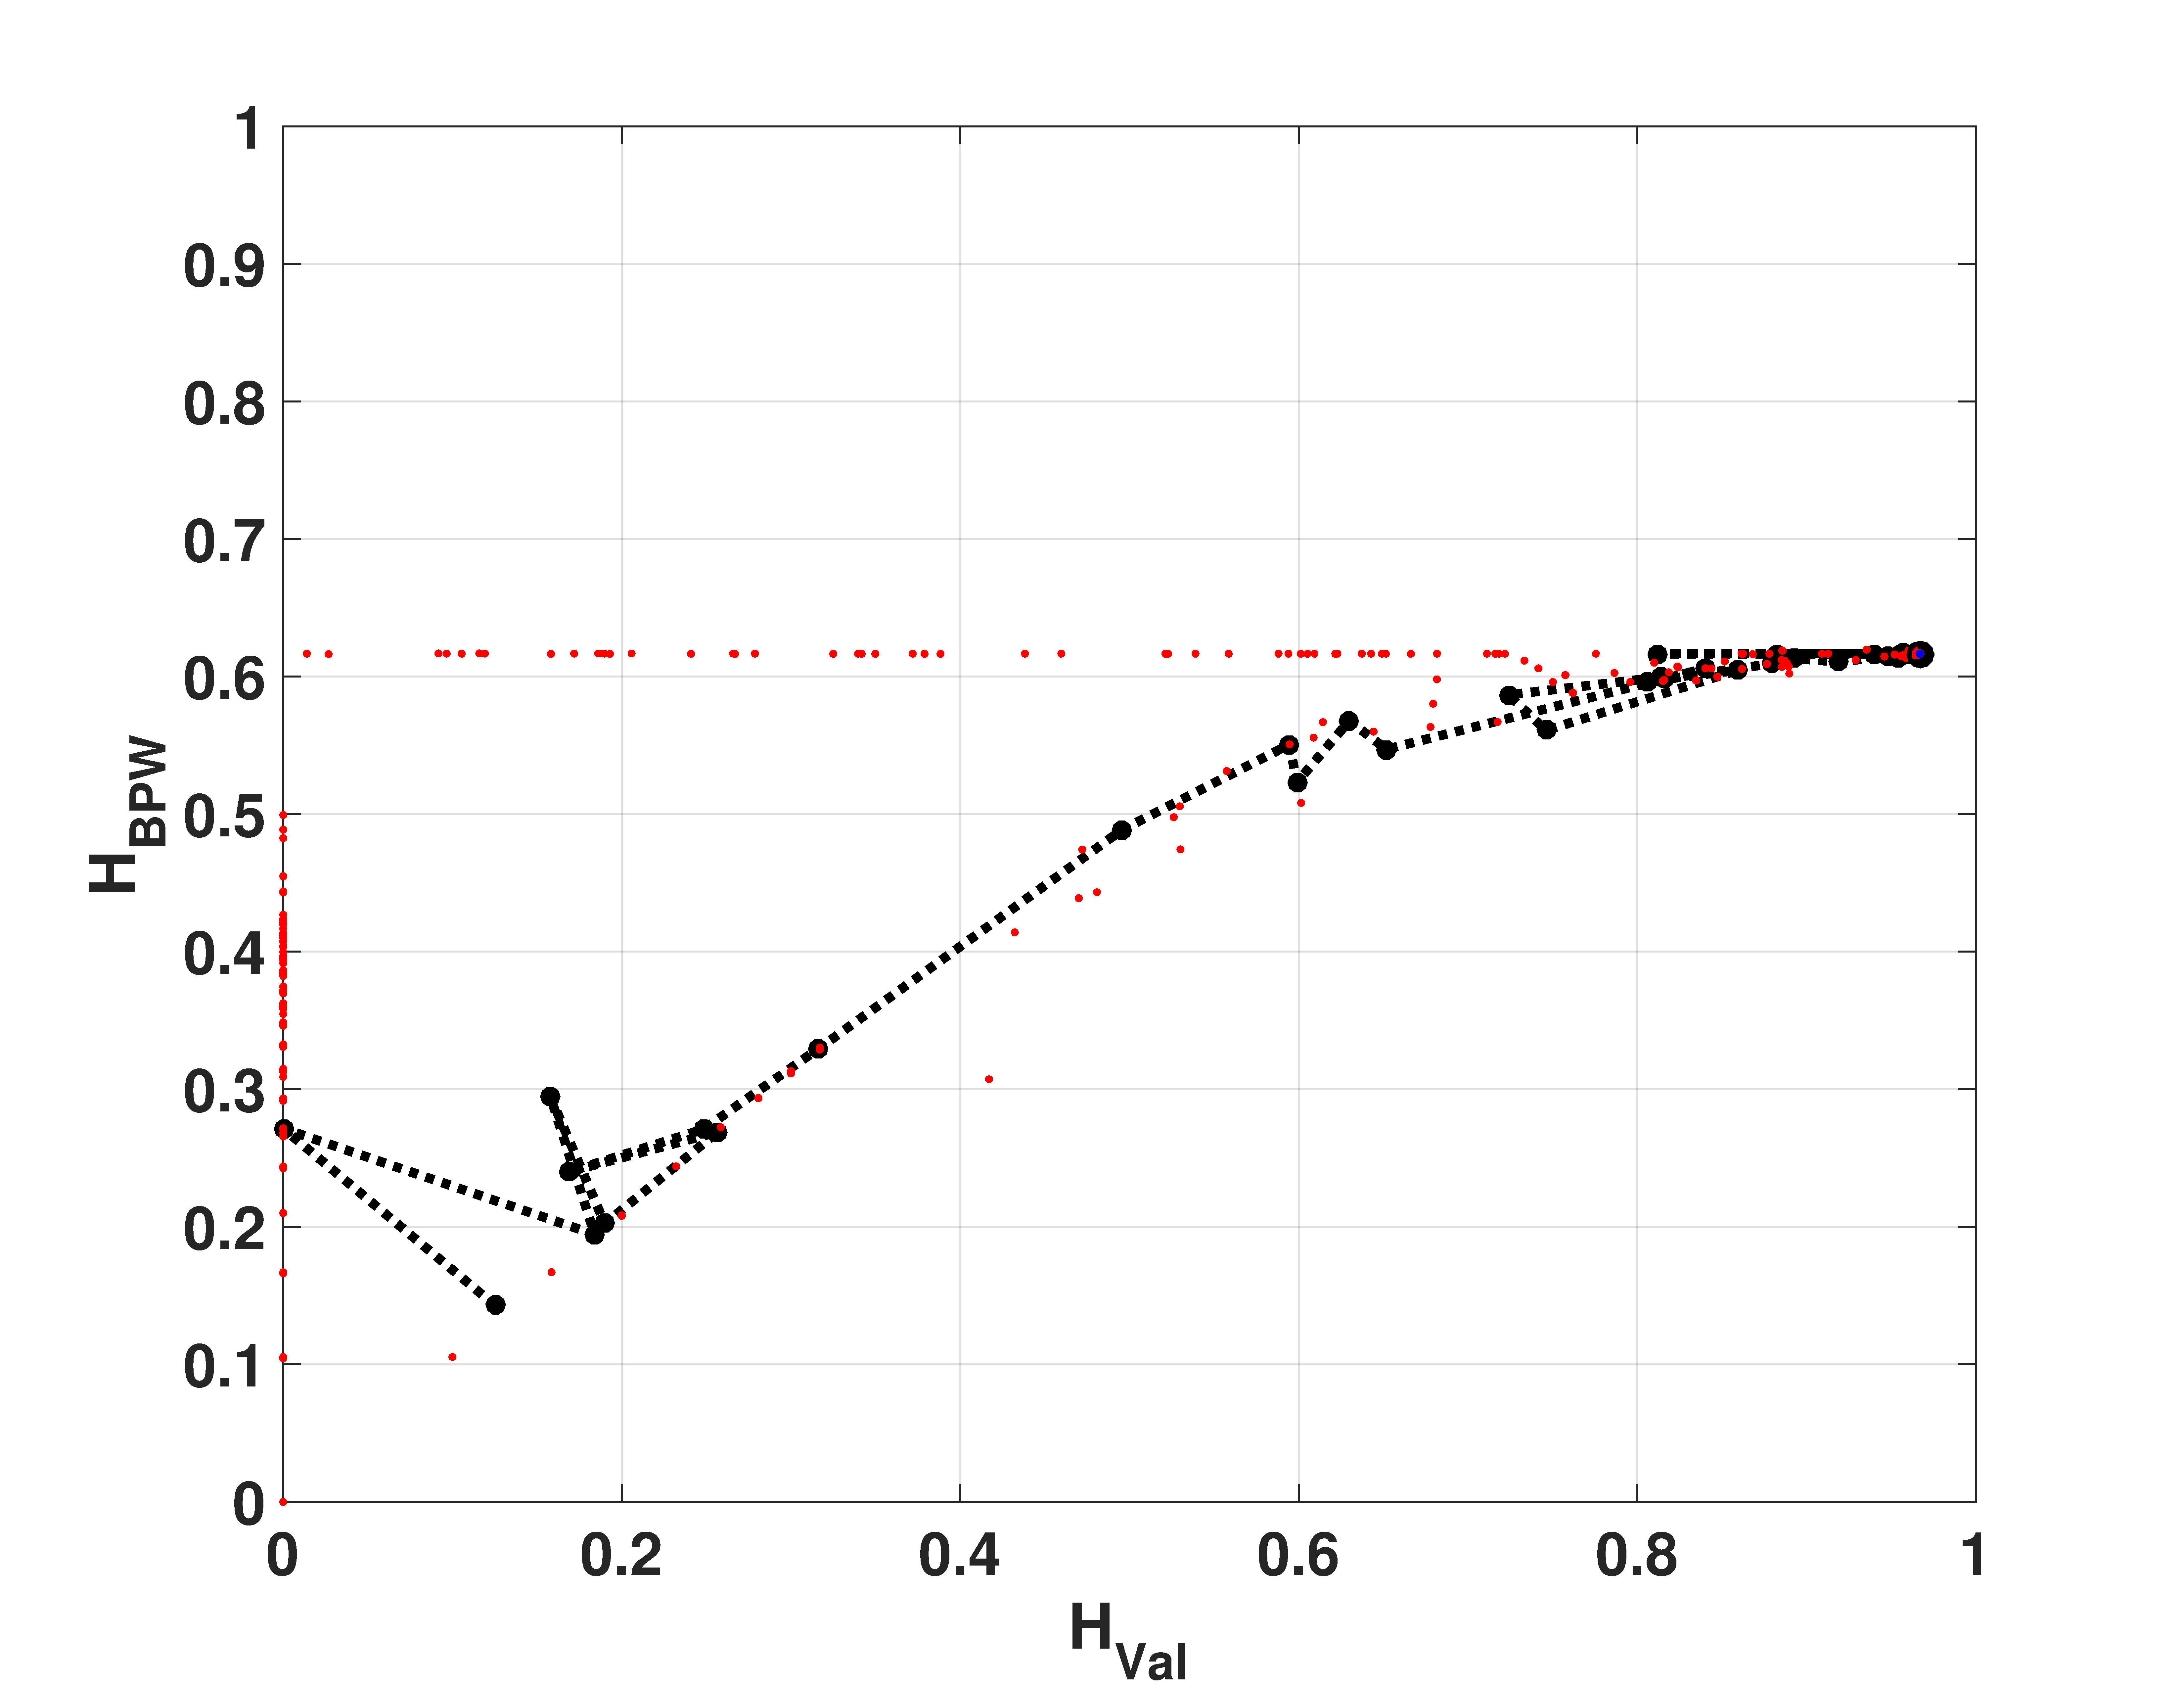
\includegraphics[width= .49\textwidth]{HbpwHval_Logistico}
	\caption{Statistical properties of the LOG map using binary representation: (a) $H_{hist}$ vs $P$ (b) $H_{BP}$ vs $P$ (c) $C_{BP}$ vs $P$ (d) Number of missing ordering patterns $MP$ vs $P$. In Figures (a) to (d) dashed line correspond to floating point numbers. (d) representation in the $H_{hist},H_{BP}$ plane in the the decimal numerical system.  The star represents the state for floating points numbers. (e) representation in the $H_{hist},H_{BP}$ plane. The star represents the state for floating point numbers; (f) representation in the $H_{BP},C_{BP}$ plane.  The star represents the state for floating points numbers. (f) representation in the $H_{BP},C_{BP}$ plane for binary numerical system.  The star represents the state for floating points numbers. } \label{fig:LOG_HH}
\end{figure}

In Fig. \ref{fig:LOG_HC} we shows the entropy-complexity planes.
Dotted gray lines are the superior and inferior margins, is spected that an chaotic system remain near superior margin.
There results characterize an chaotic behaviour, in $H_{BP}-C_{BP}$ plane we can see a low entropy and high complexity.

\begin{figure}
	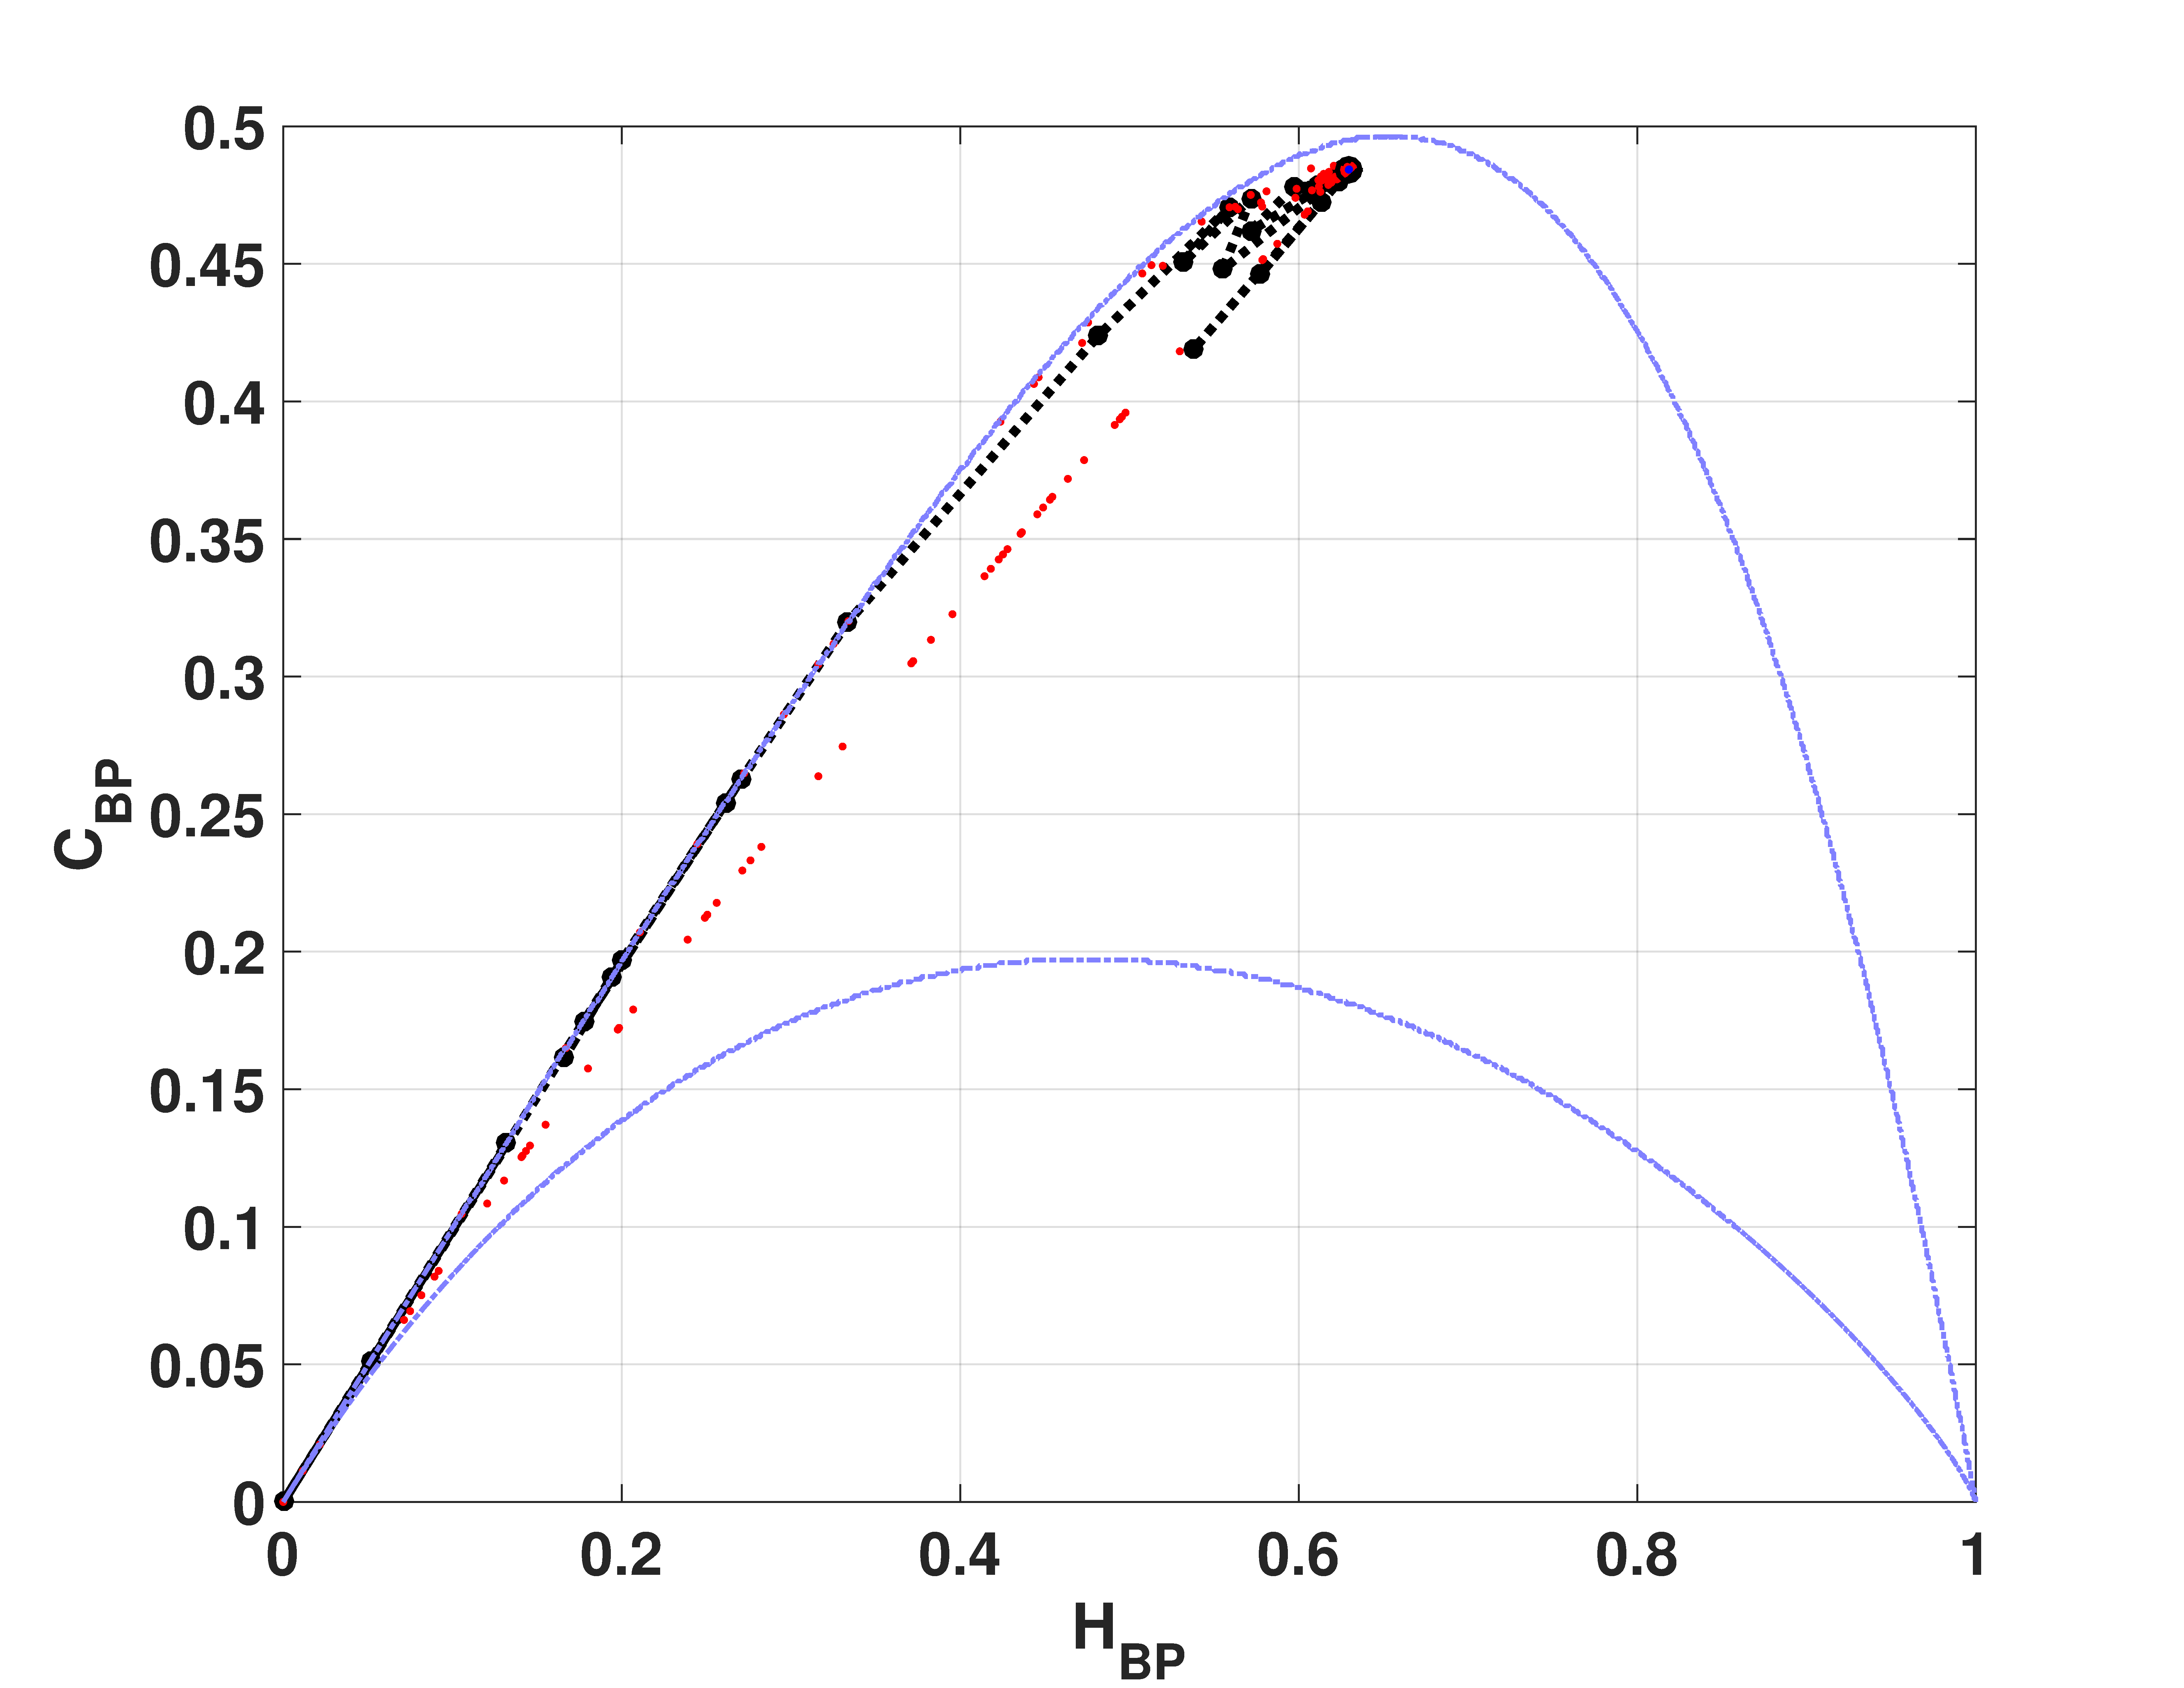
\includegraphics[width= .49\textwidth]{CbpHbp_Logistico}
	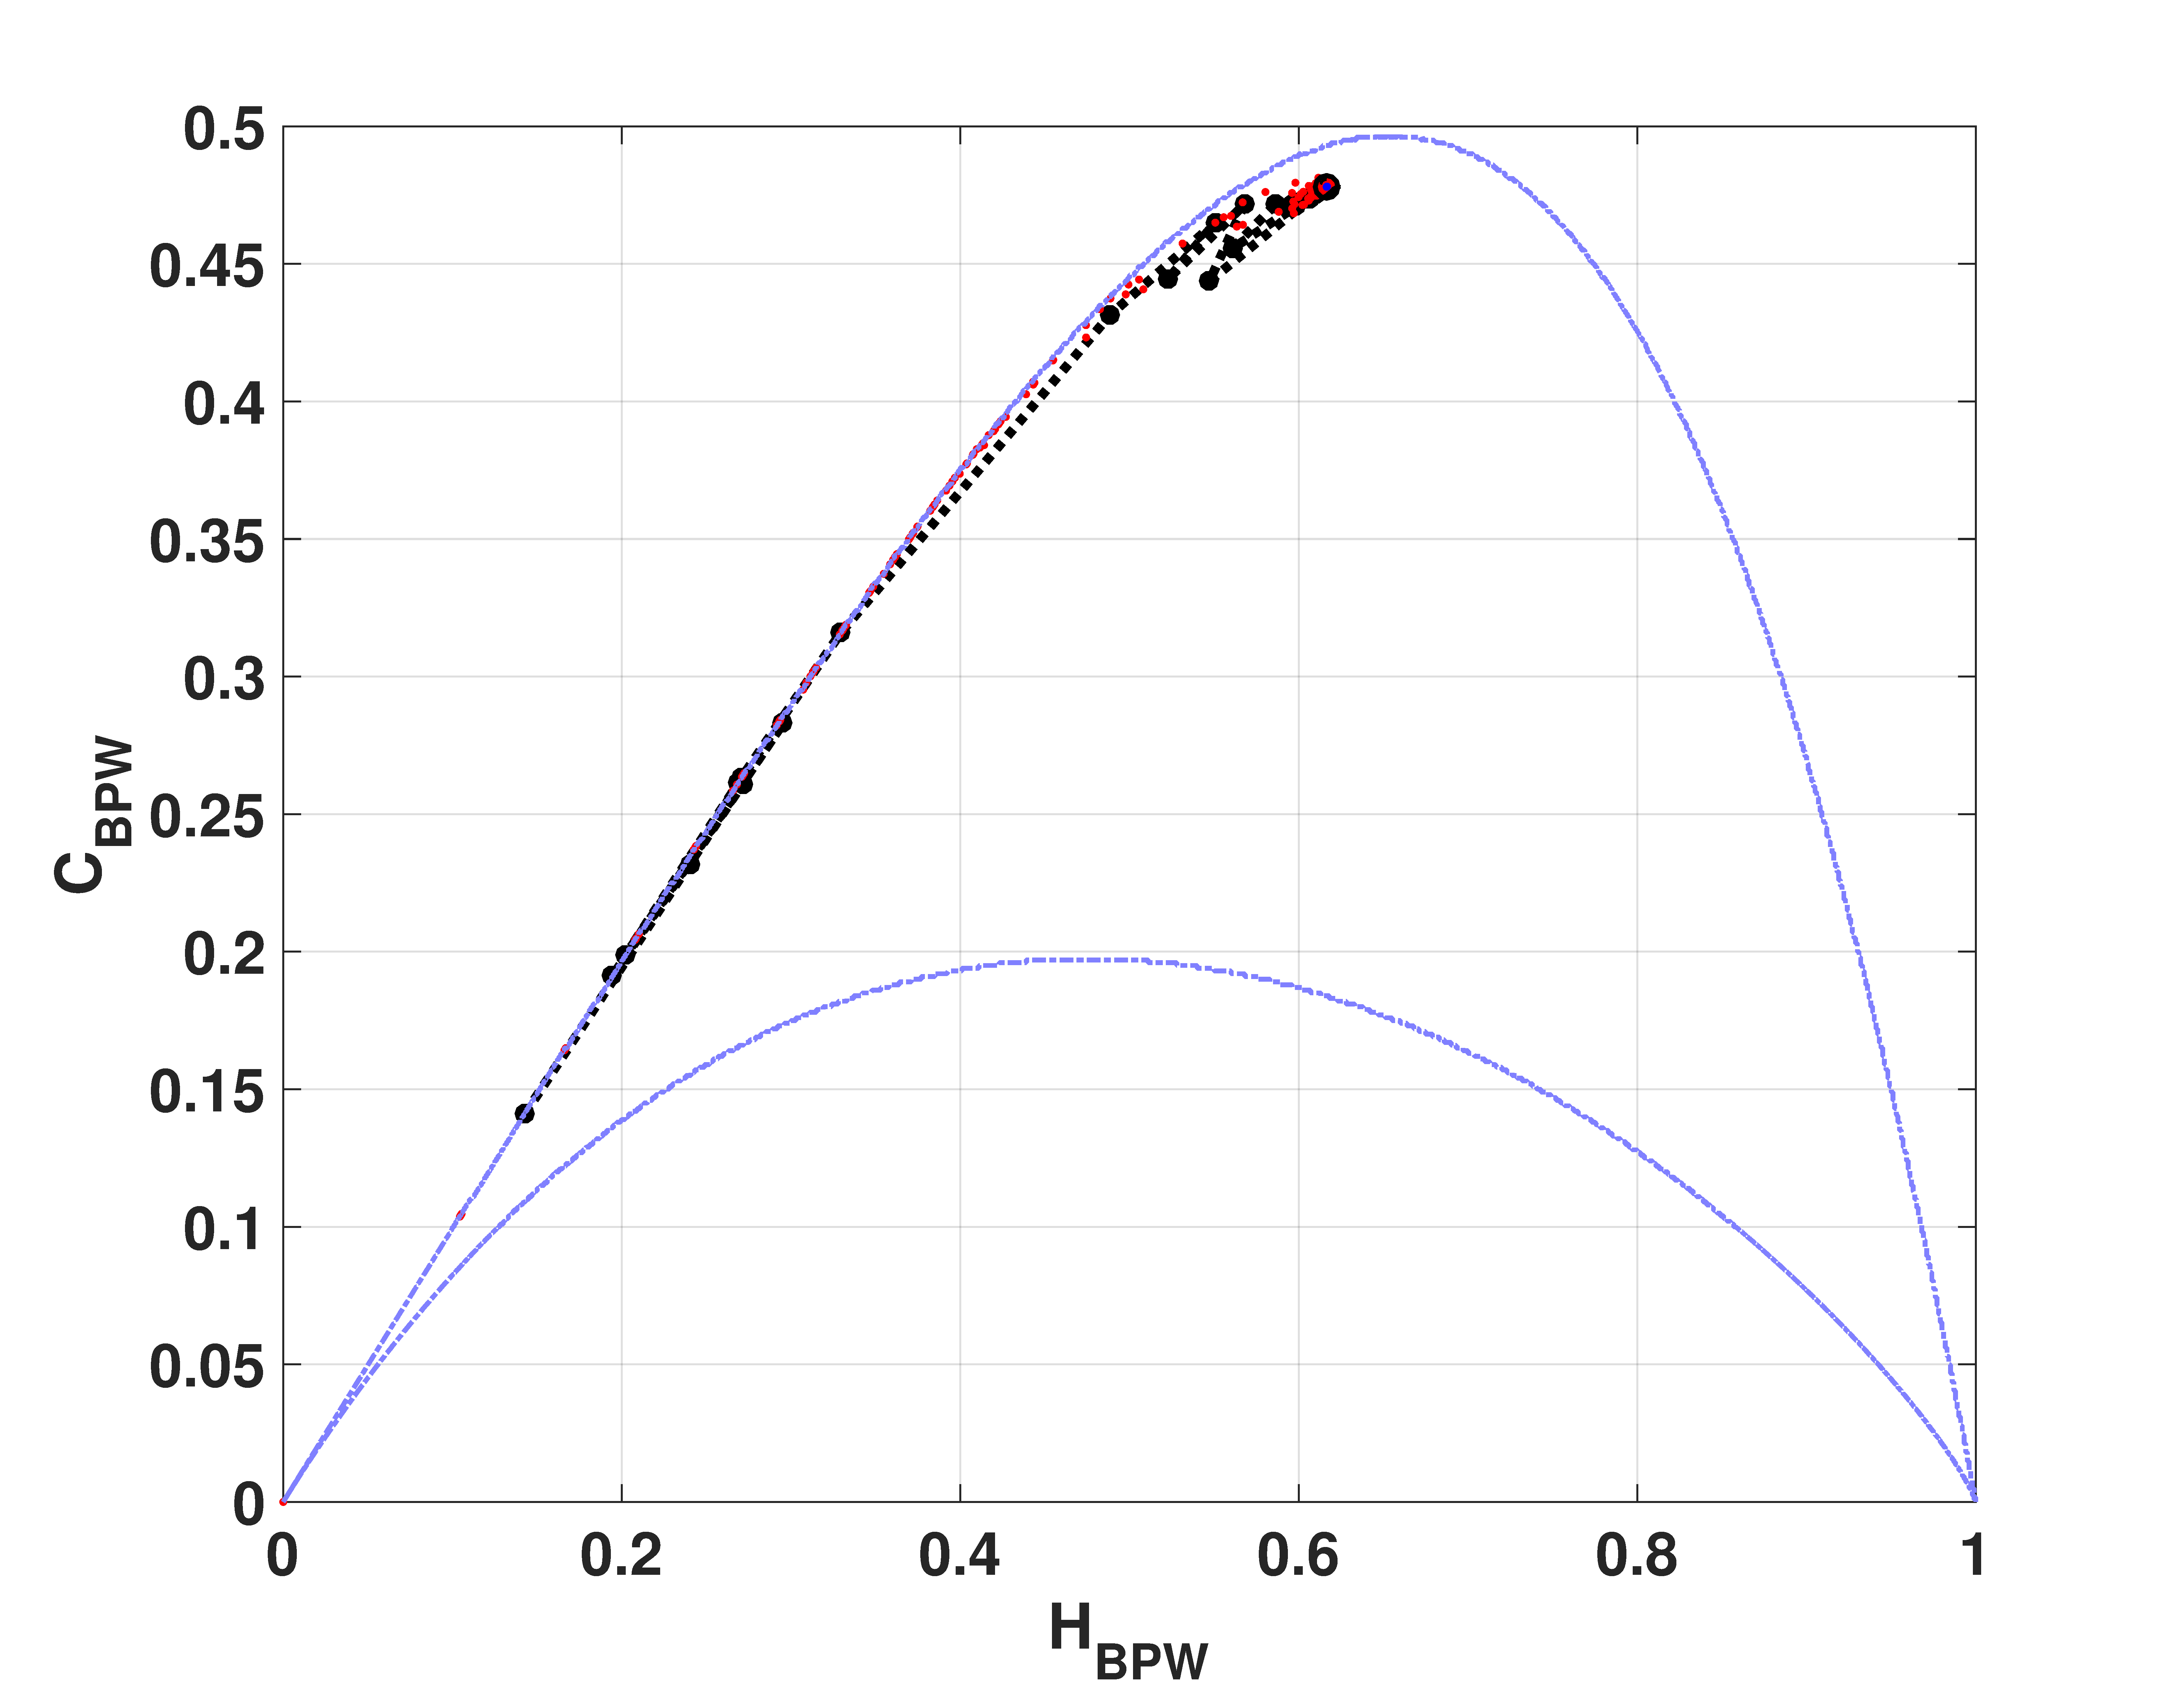
\includegraphics[width= .49\textwidth]{CbpwHbpw_Logistico}
	\caption{Statistical properties of the LOG map using binary representation: (a) $H_{hist}$ vs $P$ (b) $H_{BP}$ vs $P$ (c) $C_{BP}$ vs $P$ (d) Number of missing ordering patterns $MP$ vs $P$. In Figures (a) to (d) dashed line correspond to floating point numbers. (d) representation in the $H_{hist},H_{BP}$ plane in the the decimal numerical system.  The star represents the state for floating points numbers. (e) representation in the $H_{hist},H_{BP}$ plane. The star represents the state for floating point numbers; (f) representation in the $H_{BP},C_{BP}$ plane.  The star represents the state for floating points numbers. (f) representation in the $H_{BP},C_{BP}$ plane for binary numerical system.  The star represents the state for floating points numbers. } \label{fig:LOG_HC}
\end{figure}
